\documentclass[12pt,a4paper]{book}

\usepackage[left=2cm,right=2cm,top=2.5cm,bottom=2.5cm,ignorefoot=true]{geometry}

\setlength{\parindent}{2em}
\setlength{\parskip}{0.5em}
\renewcommand{\baselinestretch}{1.25}

\usepackage{fancyhdr}
\pagestyle{fancy}
\fancyhead{}
\renewcommand{\sectionmark}[1]{\markright{\thesection. #1}}
\renewcommand\chaptermark[1]{\markboth{#1}{}\def\cchapter{#1}}
\fancyhead[RE]{\leftmark}
\fancyhead[LO]{\rightmark}
\fancyhead[RO,LE]{\thepage}
\fancyfoot{}
\renewcommand{\footrulewidth}{0.2pt}
\fancyfoot[C]{{\em Redes Neuronales}}

\makeatletter 
\def\clearpage{% 
	\ifvmode 
		\ifnum \@dbltopnum =\m@ne 
			\ifdim \pagetotal <\topskip 
				\hbox{} 
			\fi 
		\fi 
	\fi 
\newpage 
\thispagestyle{empty} 
\write\m@ne{} 
\vbox{} 
\penalty -\@Mi 
} 
\makeatother

\usepackage[dvips]{graphicx}
\usepackage{titlesec,color}
\usepackage[font=small,labelfont=bf]{caption}

\definecolor{gray75}{gray}{0.5}
\newcommand{\hsp}{\hspace{20pt}}
\titleformat{\chapter}[hang]{\huge\bfseries}{\thechapter\hsp\textcolor{gray75}{$|$}\hsp}{0pt}{\huge\bfseries}

\usepackage[utf8]{inputenc}
\usepackage[spanish]{babel}
\usepackage{amssymb,amsfonts,latexsym,amsmath,amscd}
\usepackage{lmodern}
%\usepackage{tcolorbox}

%---------------
% Environments
\usepackage{amsthm}
\usepackage[most,theorems]{tcolorbox}
\definecolor{block-gray}{gray}{0.85}
\newtcolorbox{blockquote}{colback=block-gray,grow to right by=-1mm,grow to left by=-1mm,boxrule=0pt,boxsep=0pt,breakable}

\newtcbtheorem[number within=section]%
{definicion} % \begin..
{Definición} % Title
{fonttitle=\bfseries,colframe=red!75!black,colback=red!5!white} % Style 
{def} % label prefix; cite as ``def:yourlabel''

\newtcbtheorem[number within=section]%
{teorema} % \begin..
{Teorema} % Title
{fonttitle=\bfseries,colframe=blue!75!black,colback=blue!5!white} % Style 
{teo} % label prefix; cite as ``teo:yourlabel''

\newtcbtheorem[number within=section]%
{proposicion} % \begin..
{Proposición} % Title
{fonttitle=\bfseries,colframe=blue!75!black,colback=blue!5!white} % Style 
{prop} % label prefix; cite as ``prop:yourlabel''

\newtcbtheorem[number within=section]%
{corolario} % \begin..
{Corolario} % Title
{fonttitle=\bfseries,colframe=blue!75!black,colback=blue!5!white} % Style 
{cor} % label prefix; cite as ``cor:yourlabel''

\newtcbtheorem[number within=section]%
{notacion} % \begin..
{Notación} % Title
{fonttitle=\bfseries,colframe=green!75!black,colback=green!5!white} % Style 
{nota} % label prefix; cite as ``nota:yourlabel''

\newtcbtheorem[number within=section]%
{lema} % \begin..
{Lema} % Title
{fonttitle=\bfseries,colframe=yellow!75!black,colback=yellow!5!white} % Style 
{lema} % label prefix; cite as ``nota:yourlabel''

%-----------------------

\providecommand{\der}[1]{#1^{\prime}}
\providecommand{\abs}[1]{\lvert#1\rvert}
\providecommand{\norm}[1]{\lVert#1\rVert}
\providecommand{\inp}[1]{\langle#1\rangle}
\providecommand{\conj}[1]{\lbrace#1\rbrace}
\providecommand{\mx}[1]{max\lbrace#1\rbrace}
\providecommand{\mn}[1]{min\lbrace#1\rbrace}
\providecommand{\Lah}{L_{a}^{1}(h)}
\providecommand{\mlp}[1]{\textsl{MLP}(\rho,d,#1)}

\title{%
\textsc{Teoría Matemática de Redes Neuronales}\\[0.5em]
\large Notas de Clase%
}
\author{%
Miguel Arturo Ballesteros Montero\\[0.5em]
Facultad de Ciencias, UNAM%
}
\date{Noviembre, 2020}

%----------------------------------------

\begin{document}

\maketitle

\tableofcontents

\chapter*{Prólogo}
\addcontentsline{toc}{chapter}{Prólogo}

Durante miles de años, hemos intentado comprender como pensamos, la historia nos ha regalado grandes pensadores que han tratado de estructurar de diversas formas el complejo organismo que somos, la inteligencia artificial intenta ir un paso más allá, intenta no solo comprender si no también construir entidades inteligentes. La inteligencia Artificial es uno de los campos más nuevos de la ciencia y la ingeniería que encontró su origen poco después de la Segunda Guerra Mundial.


\section*{ Inteligencia Artificial a traves del tiempo:}
\begin{enumerate}
\item[•] \textbf{1943-1955:} La gestación de la inteligencia artificial.
 \begin{enumerate}
  \item[$\circ$] Modelo de neuronas artificiales de Warren McCulloch y Walter Pitts en 1943.
  \item[$\circ$] Turing dio conferencias sobre IA desde 1947.
 \end{enumerate}
\item[•] \textbf{1956:} El nacimiento de la inteligencia artificial.
 \begin{enumerate}
 \item[$\circ$] John MaCarthy convenció a Marvin Minsky, Claude Shannon y Nathaniel Rochester para que lo ayudaran a reunir investigadores estadounidenses interesados en la teoría de autómatas, las redes neuronales y el estudio de la inteligencia en un taller de dos meses en Dartmouth.
 \end{enumerate}
\item[•] \textbf{1952-1969:} Entusiasmo inicial, grandes exprectativas.
 \begin{enumerate}
 \item[$\circ$] Primeros solucionadores de problemas, jugadores de juegos, probadores de teoremas.
 \item[$\circ$] John McCarthy se refirió a este periodo como el ``¡Mira mama, sin manos!"
 \item[$\circ$] Creación de LISP
 \item[$\circ$] \textsl{Perceptron} de Frank Rosenblatt en 1958.
 \item[$\circ$] Adalines (\textsl{Adaptive Linear Neuron}) de Bernie Widrow y Marcian Hoff en 1960.
 \end{enumerate}
\item[•] \textbf{1966-1973} Una dosis de realidad.
 \begin{enumerate} 
 \item[$\circ$] Prueba y error: explosión combinatoria.
 \item[$\circ$] Falta de recursos computacionales. 
 \end{enumerate}
\item[•] \textbf{1969-1979:} Sistemas basados en el conocimiento ¿La clave del poder?
 \begin{enumerate}
 \item[$\circ$] Algoritmos que utilizan conocimientos específicos de dominio en lugar de solucionadores de propósito general.
 \item[$\circ$] Sistemas expertos para diagnóstico médico.
 \item[$\circ$] Incorporación de incertidumbre.
 \end{enumerate}
\item[•] \textbf{1980-presente:} La IA se convierte en industria.
 \begin{enumerate}
 \item[$\circ$]Optimización de la logística.
 \item[$\circ$]Auge repentino, pero solo unos pocos proyectos estuvieron a la altura de las expectativas.
 \item[$\circ$]Invierno IA.
 \end{enumerate}    
\item[•] \textbf{1986-presente:} El regreso de las redes neuronales:
 \begin{enumerate}
 \item[$\circ$] El algoritmo de retropropagación para entrenar redes neuronales se reiventó en ``Learning Representation by Back-Propagating Errors." Por David E. Rumelhart, Geoffrey E. Hinton y Ronald J. Williams.
 \end{enumerate}
\item[•] \textbf{1987-presente:} La IA adopta el método científico.
 \begin{enumerate}
 \item[$\circ$] Modelos ocultos de Markov.
 \item[$\circ$] Redes Bayesianas.
 \end{enumerate}
\item[•] \textbf{1995-presente}
 \begin{enumerate}
 \item[$\circ$] Internet impulsa el desarrollo de agentes inteligentes, por ejemplo:
  \begin{enumerate}
   \item[•] Chatbots.
   \item[•] Sistemas de recomendación.
   \item[•] Recomendaciones de amistades.
  \end{enumerate}
  \item[$\circ$] Acceso a recursos de computación a suficiente velocidad.
  \item[$\circ$] La era del \textsl{Big Data:} Gran cantidad de \textsl{label training data}, por ejemplo:
  \begin{enumerate}
    \item[•] Diccionarios.
    \item[•] Wordnets.
    \item[•] Wikipedia.
    \item[•] Google.
 \end{enumerate}
 \item[$\circ$] Los fundadores de la IA descontentos con su estado actual:
  \begin{enumerate}
   \item[•] La IA debería volver a sus raíces de luchar por, en palabras de Herbert Simon, ``Maquinas que piensan, que aprenden y crean".
  \end{enumerate}
  \item[$\circ$] La IA en la cultura popular.
   \begin{enumerate}
   \item[•] Lucha contra el spam.
   \item[•] Reconocimiento de voz: Siri, Alexa, Cortana.
   \item[•] Reconocimiento facial: Facebook, Apple Photos, Google Photos.
   \item[•] \textsl{Deep Blue vs Garry Kasparov}.
   \item[•] Planificación y programación autónoma: Mars rover de la NASA.
   \item[•] Vehículos robóticos: EL automóvil autónomo de Tesla.
   \item[•] Traducción automática: Traductor de Google.
   \end{enumerate}  
\end{enumerate}
\item[•] \textbf{Hoy} Tu empiezas a leer estas notas.
\end{enumerate}

\chapter{¿Que es la Inteligencia Artificial?}

  \section{Definiciones Históricas}
  \subsection{Actuar Humanamente: El enfoque de la prueba de Turing}
  
\begin{blockquote}
``El arte de crear maquinas que realizen funciones que requieren inteligencia cuando las personas lo ejecuten"

\noindent\hfill
Kurzweil, 1990
\end{blockquote}
\bigskip

\begin{blockquote}
``El estudio de hacer a las computadoras hacer cosas en las que de momento, somos mejores."

\noindent\hfill
Rich and Knight, 1991
\end{blockquote}
\bigskip

En 1950 Turing ideo una prueba para proporcionar una definición operativa satisfactoria de inteligencia; Una computadora pasa la prueba si un interrogador humano, después de formular algunas preguntas escritas, no puede decir si las respuestas escritas provienen de una persona o una computadora.
\bigskip

La computadora debe poseer las siguientes características:
\begin{enumerate}
\item[•] \textbf{Procesamiento del lenguaje natural:} para comunicarse, por ejemplo en inglés.
\item[•] \textbf{Representación del conocimiento:} para almacenar información
\item[•] \textbf{Razonamiento automatizado:} utilizar la información almacenada, responder preguntas y sacar conclusiones
\item[•] \textbf{Aprendizaje automático:} adaptarse a nuevas circunstancias, extrapolar y detectar patrones.
\end{enumerate}
La prueba de Turing sigue siendo relevante incluso hoy, pero menos desde la ingeniería y más desde la postura filosófica, en ejemplo parecido sería:
\begin{enumerate}
\item[•] La busqueda del ``vuelo artificial'' tuvo éxito cuando los hermanos Wright y otros dejaron de imitar a las aves y comenzaron a usar túneles de viento y aprender sobre aerodinámica.
\item[•] Los textos de ingeniería aeronáutica no definen el objetivo de su campo como fabricar ``Máquinas que vuelan tan exactamente como las palomas que pueden engañar incluso a otras palomas"
\end{enumerate}
\subsection{Pensar Humanamente: El enfoque de modelado  cognitivo}

\begin{blockquote}
``El nuevo y emocionante esfuerzo de hacer que las computadoras piensen [...] maquinas con mentes, en el sentido completo y literal."

\noindent\hfill
Haugeland, 1985
\end{blockquote}
\bigskip

\begin{blockquote}
``[La automatización de] actividades que asociamos con el pensamiento humano, actividades como la toma de decisiones, la resolución de problemas, el aprendizaje [...]"

\noindent\hfill
Bellman, 1978
\end{blockquote}
\bigskip
Para saber si un programa ``piensa como un ser humano", debemos aprender qué es el pensamiento humano:
\begin{enumerate}
\item[•] Observa nuestros pensamientos a medida que pasan
\item[•] Observar a las personas durante una tarea
\item[•] Experimentos psicológicos/neurocientíficos
\end{enumerate}
Sin embargo, para nuestro esfuerzo, será una buena práctica mantener separados los campos como la ciencia cognitiva, la neurociencia, la psicología y la filosofía el mayor tiempo posible.
\subsection{Actuar Racionalmente: El enfoque del agente racional}

\begin{blockquote}
``La Inteligencia Computacional es el estudio del diseño de agentes inteligentes"

\noindent\hfill
Poole et al., 1998
\end{blockquote}
\bigskip

\begin{blockquote}
``IA [...] se preocupa por el comportamiento inteligente de los artefactos"

\noindent\hfill
Nilsson, 1998
\end{blockquote}
\bigskip

Crear agentes (por ejemplo, programas informáticos) que operen de forma autónoma, perciban su entorno, persistan durante un período de tiempo prolongado, se adapten al cambio, creen,  persigan metas. Hacer inferencias es el caso extremo de ser un agente racional.\bigskip

En muchas ocasiones, sin embargo, no es posible realizar inferencias correctas, por ejemplo:
\begin{enumerate}
\item[•] Comprensión insuficiente del medio ambiente
\item[•] No hay suficientes datos de entrada para basar una decisión
\end{enumerate}
Un agente racional es aquel que actúa para lograr el mejor resultado ó, cuando hay incertidumbre, el mejor resultado esperado.\\
\\
De esta forma, el estándar de racionalidad está matemáticamente bien definido y es completamente general (como mostraremos en la siguiente sección con el enfoque de ``Las leyes del pensamiento"), por otro lado el comportamiento humano, esta bien adaptado para un entorno específico y se define a si mismo por la suma total de todas las cosas que hacen los humanos.
\subsection{Pensar Racionalmente: El enfoque de las leyes del pensamiento}
Un uso de razonamiento lógico y argumentación, por ejemplo:
\begin{enumerate}
\item[•] \textbf{Deducción:} Una regla general aplicada a un caso particular implica un resultado trivial.
\begin{center}
\begin{tabular}{|l|l|l|}
\hline 
\textbf{Entrada} & \textbf{Implicación} & \textbf{Ejemplo} \\ 
\hline 
REGLA &  & En un planeta, su sol sale todos los días \\ 
\hline 
CASO &  & Estamos en un planeta \\ 
\hline 
 & RESULTADO & El sol sale todos los dias \\ 
\hline 
\end{tabular} 
\end{center}
El reino de las matemáticas.
\item[•] \textbf{Inducción} de un resultado trivial en un caso particular esperamos inferir la regla general.
\begin{center}
\begin{tabular}{|l|l|l|}
\hline 
\textbf{Entrada} & \textbf{Implicación} & \textbf{Ejemplo} \\ 
\hline 
RESULTADO &  & El sol salía todos los días \\ 
\hline 
CASO &  & Estamos en un planeta \\ 
\hline 
 & REGLA & En un planeta, su sol sale todos los días \\ 
\hline 
\end{tabular} 
\end{center}
El reino de la ciencia.
\item[•] \textbf{Secuestro:} De una regla general y un resultado trivial esperamos inferir el caso particular 
\begin{center}
\begin{tabular}{|l|l|l|}
\hline 
Entrada & Implicación & Ejemplo \\ 
\hline 
REGLA &  & En un planeta, su sol sale todos los días \\ 
\hline 
RESULTADO &  & El sol salía todos los días \\ 
\hline 
 & CASO & Estamos en un planeta \\ 
\hline 
\end{tabular} 
\end{center}
Más raramente utilizado.
\end{enumerate}
\section{¿Que es el Machine Learning?}
\begin{blockquote}
``[Machine Learning] brinda a las computadoras la capacidad de aprender sin estar programada explicitamente."

\noindent\hfill
Samuel, 1959
\end{blockquote}
\bigskip

Dicho de otra manera, el Machine Learning es un sub-campo de la Inteligencia Artificial en donde se buscan algoritmos ``suaves" que, hasta cierto punto, pueden adaptarse a un cierto tipo de tarea en lugar de consistir simplemente en una lógica codificada. que busca manejar grandes cantidades de datos y realizar por ejemplo:
\begin{enumerate}
\item[•] Estructuración de datos
\item[•] Encontrar correlaciones
\item[•] Clasificar datos
\item[•] Reconocer patrones
\item[•] Comprender datos
\item[•] Tomar decisiones basadas en datos
\item[•] Adaptar tareas a datos
\item[•] Extrapolación/ predicción
\end{enumerate} 
\subsection{Supervised Learning}
Algoritmos ``suaves" que infieren la tarea designada mediante la inspección de los datos de entrenamiento apropiados.

Ejemplos:
\begin{enumerate}
 \item[$\circ$] Clasificación: Predicción de clases discretas, por ejemplo:
 \begin{enumerate}
  \item[•] El correo electrónico es spam o no
  \item[•] Identificar imagenes borrosas
 \end{enumerate}
 \item[$\circ$] Regresión: Predicción de parámetros continuos, por ejemplo:
  \begin{enumerate}
  \item[•] Consumo de energia de acuerdo con el comportamiento del usuario aprendido
  \item[•] Predicción de una tendencia según una historia determinada.
  \end{enumerate}
\end{enumerate}

\begin{figure}[hbtp]
\centering
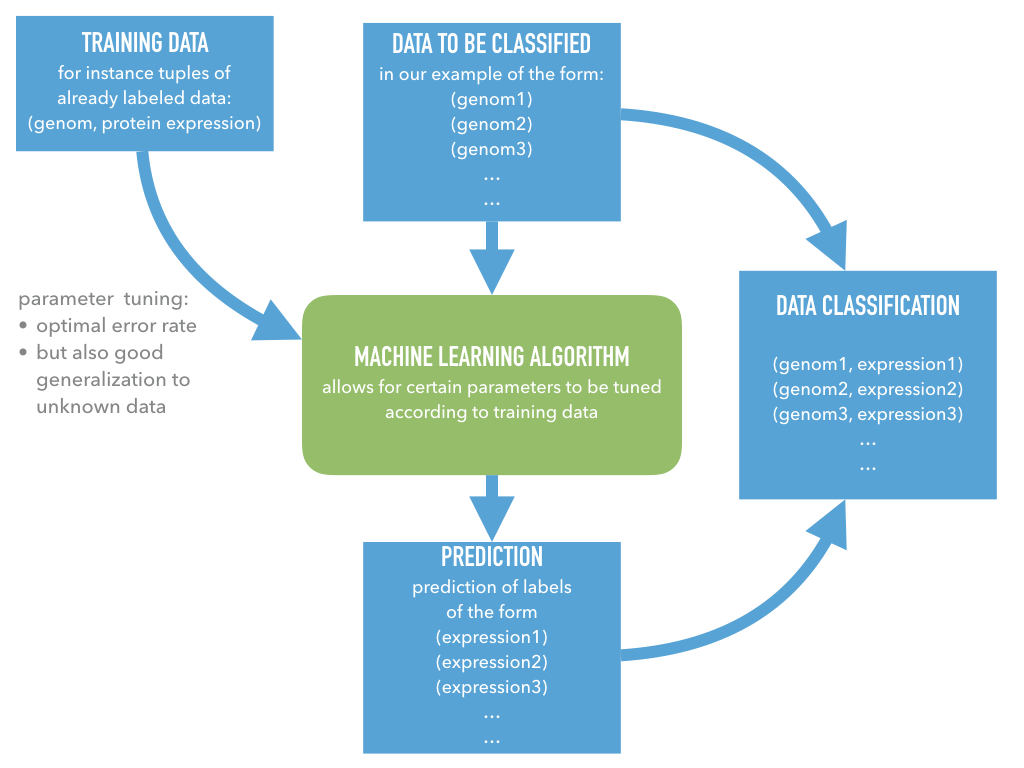
\includegraphics[scale=0.4]{Graficas/SL_1.jpg}
\caption{Algoritmo Machine Learning}
\end{figure}

\subsection{Unsupervised Learning}
Estructurar los datos en grupos sin conocimientos previos detallados.\\
\\
Ejemplos:
\begin{enumerate}
 \item[$\circ$] Wordnets: relaciones entre palabras de un leguaje natural.
 \item[$\circ$] Referencias cruzadas entre documentos.
 \item[$\circ$] Comprensión de datos y reducción de dimensionalidad.
\end{enumerate}

\begin{figure}[hbtp]
\centering
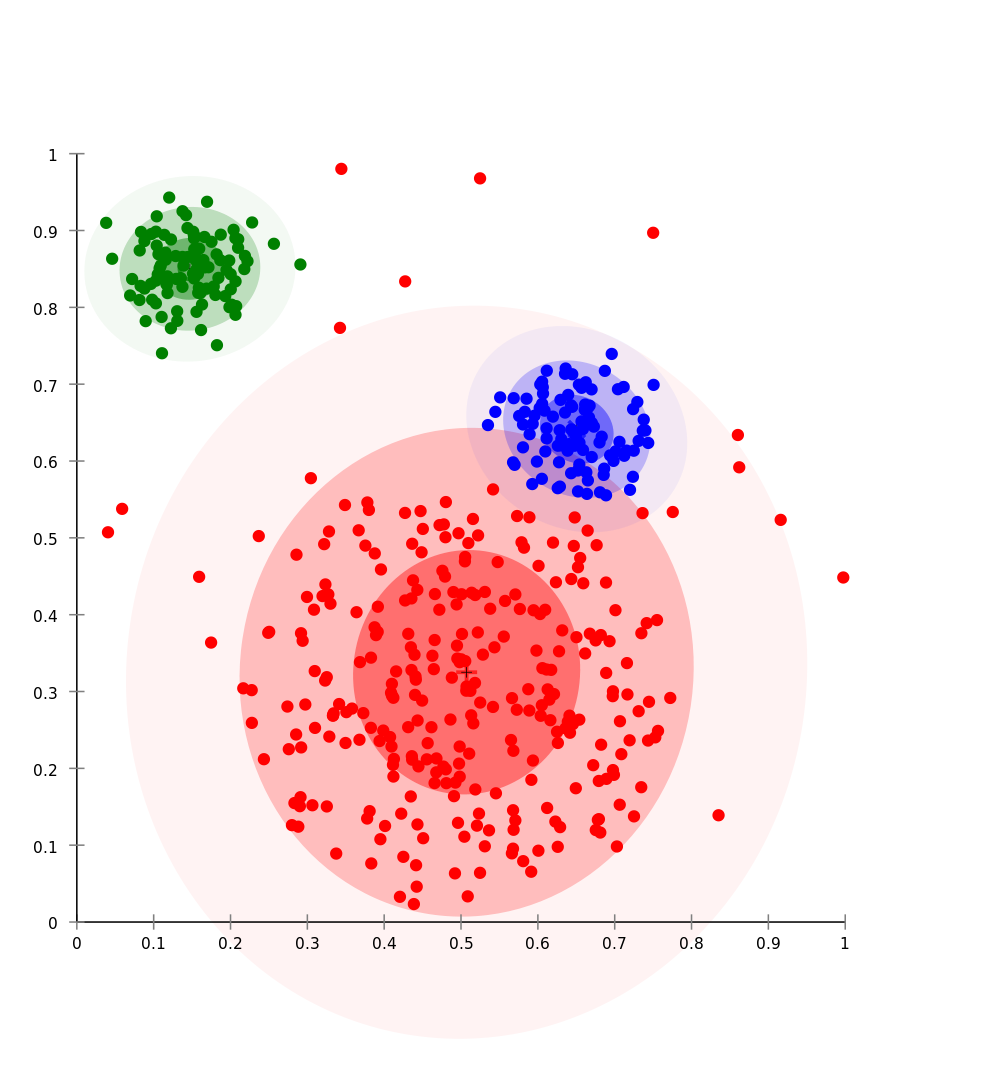
\includegraphics[scale=0.35]{Graficas/cluster_example.png}
\caption{Ejemplo ficticio de puntos de datos 2D. El color indica una relación entre los puntos de datos. A partir de estas relaciones, las regiones sombreadas pueden inferirse mediante un algoritmo de aprendizaje automático no supervisado. Esto puede ser util cuando se buscan propiedades estructuradas burdas de un conjunto de datos}
\end{figure}
\subsection{Reinforcement Learning}
Un agente (Machine Learning program + artifact) aprende a realizar una determinada tarea mediante, por ejemplo, prueba y erros. El aprendizaje se ve facilitado por la capacidad de observar el entorno y recibir retroalimentación en función de las acciones.\\
Ejemplos:
\begin{enumerate}
 \item[$\circ$] Movimiento de un robot en terreno desconocido o bajo condiciones variables
 \item[$\circ$] Obteniendo puntueciones altas en juegos de Atari como \textsl{Google depmind}
\end{enumerate}

\begin{figure}[hbtp]
\centering
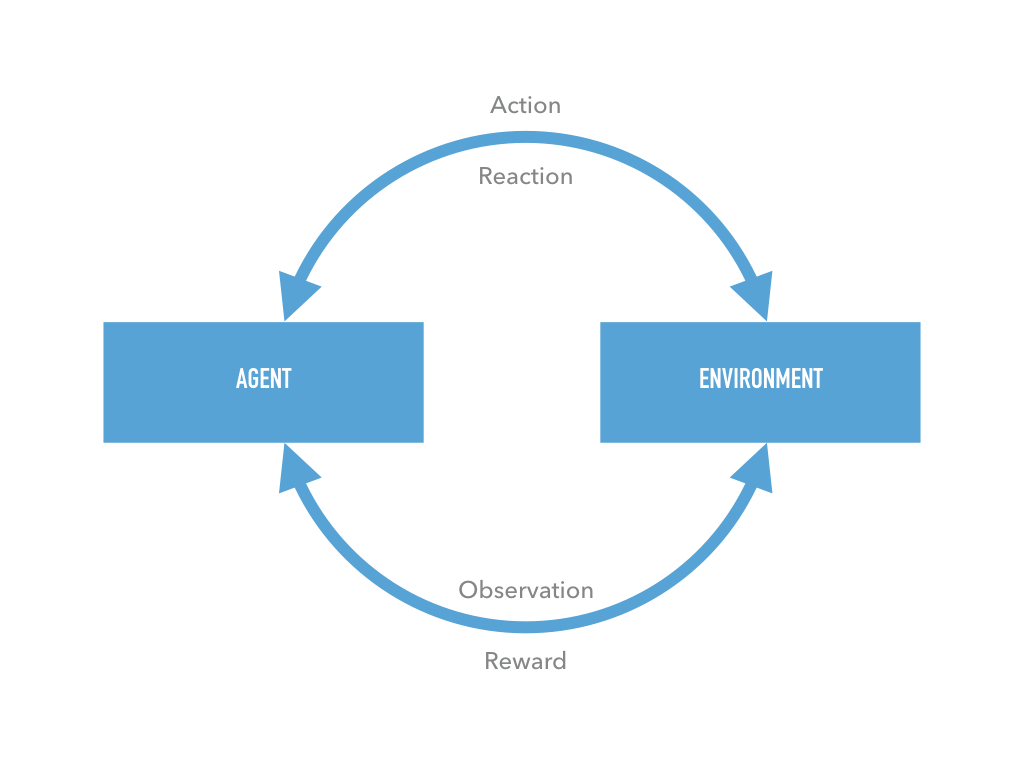
\includegraphics[scale=0.2]{Graficas/DL_1.jpg}
\caption{a}
\end{figure}
\part{Clases}
\chapter{Neuronas y Redes Neuronales}
  
En este curso estudiaremos objetos matemáticos llamados redes neuronales. Estos son elementos centrales en IA (Inteligencia Artificial).

La primera neurona en el contexto del cerebro fue propuesta por McCulloch y Pitts en 1943.
\begin{equation}\label{eq:McCulloch-Pitts}
\mathbb{R}^{d}\ni \widehat{x}\rightarrow \chi_{\mathbb{R}^{+}}\left(\sum w_{i}x_{i}-\theta\right),
\end{equation}
en donde:
\begin{itemize}
\item $d\in\mathbb{N}$.
\item Para todo conjunto A.
\begin{equation*}
 \chi_{A}(y)=
\begin{cases}
1 & \text{ si $y\in A$, }\\ 
0 & \text{ si $y\not\in A$. }  
\end{cases}
\end{equation*}
\item $\mathbb{R}^{+}=[0,\infty]$.
\item $w_{i}\in\mathbb{R}, \forall i$ := Pesos
\item $\theta\in\mathbb{R}$:= Umbral
\item $\chi_{\mathbb{R}^{+}}$ := Función de activación.
\item $\widehat{x}=\begin{pmatrix}
x_{1} \\ 
\vdots \\ 
x_{d}
\end{pmatrix}$
\end{itemize}
Si la combinación lineal $\sum x_{i}w_{i}$ es mayor que $\theta$, entonces la neurona se activa, de lo contrario no lo hace.

La función:
\begin{equation}
\widehat{x}=
\begin{pmatrix}
x_{1} \\ 
\vdots \\ 
x_{d} \\ 
\end{pmatrix}
\rightarrow \sum x_{i}w_{i}-\theta     
\end{equation}
es una transformación afín (una transformación lineal compuesta con una traslación) y la función $\chi_{\mathbb{R}^{+}}$ es una función no lineal.

De forma mas general, definimos una neurona como una transformación afin compuesta con una función no lineal, es decir:


\begin{definicion}{Neurona}{neurona}
Sea una transformación afin $T:\mathbb{R}^{m}\rightarrow \mathbb{R}^{n}$ y una función no lineal $\rho:\mathbb{R}\rightarrow\mathbb{R}$. Definimos una {\bf neurona} como la composición:
\begin{equation}
\begin{split}
\mathbb{R}^{m}\ni 
\widehat{x}=\left(
\begin{tabular}{c}
$x_{1}$ \\ 
$\vdots$ \\ 
$x_{m}$ \\ 
\end{tabular}
\right)
\rightarrow
\rho(T(\widehat{x})):=
\left(
\begin{tabular}{c}
$\rho(T(\widehat x)_{1})$ \\ 
$\vdots$ \\ 
$\rho(T(\widehat x)_{n})$ \\ 
\end{tabular}
\right)
\end{split}
\end{equation}
De donde:
\begin{enumerate}
\item[•] 
$T(\widehat x)=
\left(
\begin{tabular}{c}
$T(\widehat x)_{1}$ \\ 
$\vdots$ \\ 
$T(\widehat x)_{n}$ \\ 
\end{tabular}
\right)
\in\mathbb{R}^{n}
$
\item[•] $T(\widehat x)_{i}$ es la i-ésima componente de $T(\widehat{x})$
\end{enumerate}
\end{definicion}

La función $\rho$ es la función de activación y la transformación afin $T$ contiene a los pesos y al umbral (de forma abstracta).

Una red neuronal es una composición de neuronas, en nuestro caso consideramos una única función de activación para todas las neuronas de la red.

\begin{definicion}{Red Neuronal}{red_neuronal}
 Una red neuronal consiste en L transformaciones afines, $T_{1},T_{2},...,T_{L}$ y una función de activación $\rho:\mathbb{R}\rightarrow\mathbb{R}$, definimos la red neuronal como la composición:
 \begin{equation}
 \begin{split}
F=T_{L}\circ\rho\circ T_{L-1}\circ\rho\circ ... \circ\rho\circ T_{1} 
 \end{split}
 \end{equation}
En donde estamos identificando a la función $\rho$ con funciones $\rho:\mathbb{R}^{n}\rightarrow\mathbb{R}^{n}$ como:
\begin{center}
$\rho
\left(
\begin{tabular}{c}
$Y_{1}$ \\ 
$\vdots$ \\ 
$Y_{n}$ \\ 
\end{tabular}
\right):=
\left(
\begin{tabular}{c}
$\rho(Y_{1})$ \\ 
$\vdots$ \\ 
$\rho(Y_{n})$ \\ 
\end{tabular}
\right)
$
\end{center}
(Esto es un abuso de notación que siempre se usa)
\end{definicion}
\newpage
\begin{figure}[hbtp]
\centering
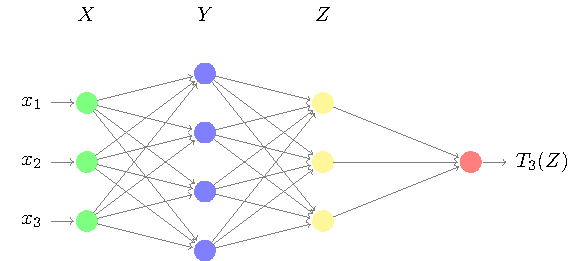
\includegraphics[scale=1.5]{Graficas/RN_1.pdf}
\caption{Ejemplo de Red Neuronal}
\end{figure}

En donde:
\begin{enumerate}
\item[•] $X=\left(\begin{matrix}
x_{1}\\
x_{2}\\
x_{3}
\end{matrix}\right)$
\item[•] $Y=\left(\begin{matrix}
y_{1}\\
y_{2}\\
y_{3}\\
y_{4}
\end{matrix}\right)=\rho(T_{1}(X))$
\item[•] $Z=\left(\begin{matrix}
z_{1}\\
z_{2}\\
z_{3}
\end{matrix}\right)=\rho(T_{2}(Y))$
\end{enumerate}

A la función $F$ se le nombra un \textbf{``Multilayer Perceptron" (MLP)} de dimensión $d$, $L$ niveles y función de activación $\rho$. donde el dominio de $T_{1}$ es $\mathbb{R}^{d}$.
\chapter{Resultados de Análisis Funcional}

\section{Espacios de Banach y Espacios de Hilbert}

\begin{definicion}{Norma}{norma}
Sea V un espacio vectorial, una norma en V es una asignación $V\ni \widehat{x}\rightarrow \lVert \widehat x \rVert$, tal que:
\begin{enumerate}
\item $\norm{\widehat{x}}\geq 0, \forall \widehat{x}$
\item $\norm{\widehat{x}}=0\Leftrightarrow \widehat{x}=\widehat{0}$
\item $\norm{\alpha\cdot\widehat{x}}=\abs{\alpha}\norm{\widehat{x}}, \forall\alpha\in\mathbb{R}$
\item $\norm{\widehat{x}+\widehat{y}}\leq\norm{\widehat{x}}+\norm{\widehat{y}}$ 
\end{enumerate}
\end{definicion}

\smallskip

\begin{definicion}{Producto Interior}{prod_int}
Sea V un espacio vectorial. un producto interior es una asignación $V\ni\widehat{x},\widehat{y}\rightarrow \inp{\widehat{x},\widehat{y}}$, tal que:
\begin{enumerate}
\item $\inp{\widehat{u}+\widehat{v},\widehat{w}}=\inp{\widehat{u},\widehat{w}}+\inp{\widehat{v},\widehat{w}}$
\item $\inp{\lambda\widehat{v},\widehat{w}}=\lambda\inp{\widehat{v},\widehat{w}}, \forall\lambda\in\mathbb{R}$
\item $\inp{\widehat{u},\widehat{v}}=\inp{\widehat{v},\widehat{u}}$
\item $\inp{\widehat{v},\widehat{v}}\geq 0, \inp{\widehat{v},\widehat{v}}=0 \Leftrightarrow \widehat{v}=0$
\end{enumerate}
\end{definicion}

\smallskip

\begin{notacion}{}{notacion_1}
Todo producto interior induce una norma de la forma:
\begin{center}
$\norm{\widehat{x}}=\sqrt{\inp{\widehat{x},\widehat{x}}}$
\end{center}
\end{notacion}

\smallskip

\begin{definicion}{Completitud}{completitud}
Decimos que un espacio vectorial normado V, es completo si toda sucesión de Cauchy converge, es decir:\\

Sea $(\widehat{v}_{n})_{n\in\mathbb{N}}$ una sucesión en V tal que $\forall\epsilon >0, \exists N\in\mathbb{N}$, tal que $\forall n,m\geq N, \norm{\widehat{v}_{n}-\widehat{v}_{m}}<\epsilon$\\

Entonces existe: $$\widehat{v}=\lim_{n\rightarrow\infty} \widehat{v}_{n}$$ 
\end{definicion}

\smallskip

\begin{definicion}{Espacios de Banach y de Hilbert}{banach_hilbert}
\begin{enumerate}
\item[•] Un espacio de Banach es un espacio vectorial normado y completo.
\item[•] Un espacio de Hilbert es una espacio vectorial con producto interior y completo.
\end{enumerate}
\end{definicion}

\smallskip

\begin{notacion}{}{notacion_2}
Sea V un espacio vectorial normado:
\begin{enumerate}
\item Bola: Sea $\widehat{x}\in V$ y $r>0$, denotamos por $B_(\widehat{x},r):=\lbrace y\in V\;|\; \norm{\widehat{y}-\widehat{x}}<r \rbrace$.
\\
\item Conjunto Abierto: Sea $A\subset V$. Decimos que A es abierto si $\forall \widehat{a}\in A, \exists r>0$ tal que $B(\widehat{a},r)\subset A$. 
\item Conjunto Cerrado: $B\subset V$. Decimos que B es cerrado si $B^{c}$ es abierto o equivalentemente si se cumple lo siguiente.
\begin{center}
Si $\widehat{y}\in V$ es tal que $\forall\epsilon >0$ tal que $B(\widehat{y},\epsilon)\cap B\neq\emptyset$, entonces $\widehat{y}\in B$.
\end{center}
\item Cerradura: Sea $C\subset V$ la cerradura es el conjunto cerrado mas chico que contiene a C. Denotamos con $\bar{C}$ a la cerradura de C. El conjunto $\bar{C}$ se caracteriza con la siguiente propiedad.
\begin{center}
$\widehat{y}\in\overline{C}\Leftrightarrow \forall\epsilon >0, B(\widehat{y},\epsilon)\cap C\neq\emptyset$.
\end{center}
Notemos que C es cerrado $\Leftrightarrow C=\overline{C}$.
\item Interior: El interior de un conjunto A es el conjunto abierto mas grande contenido en A y lo denotamos con $A^{\circ}$.
\end{enumerate}
\end{notacion}

\smallskip

\begin{definicion}{Densidad}{densidad}
Sea V un espacio vectorial normado y $M\subset V$. Decimos que M es denso si se cumple alguno de los siguientes puntos:
\begin{enumerate}
\item $\overline{M}=V$.
\item $\forall \widehat{v}\in V, \forall\epsilon >0$ tal que $B(\widehat{v},\epsilon)\cap M\neq\emptyset$.
\end{enumerate}
\end{definicion}

\smallskip

\begin{definicion}{Norma de una transformación lineal continua}{norma_transformacion}
Sean V y W espacios vectoriales normados y $\Lambda :V\rightarrow W$ una transformación lineal, definimos:
\begin{center}
$\norm{\Lambda}:= \sup\lbrace \norm{\Lambda(\widehat{v})}\;|\;\widehat{v}\in V\; y \; \norm{\widehat{v}}\leq 1\rbrace$
\end{center}
Nota: $\Lambda$ es continua $\Leftrightarrow \sup\lbrace \norm{\Lambda(\widehat{v})}\;|\;\widehat{v}\in V\; y \; \norm{\widehat{v}}\leq 1\rbrace <\infty$
\end{definicion}

\smallskip

\begin{teorema}{Hahn-Banach}{hahn-banach}
Sea V un espacio vectorial normado y $M\subset V$ un sub-espacio vectorial, supongamos $h:M\rightarrow\mathbb{R}$ es continua y lineal. entonces existe una extensión $g:V\rightarrow \mathbb{R}$ (lineal y continua) tal que:
\begin{enumerate}
\item $g(m)=h(m),\;\forall m\in M$
\item $\norm{h}=\norm{g}$ 
\end{enumerate} 
\end{teorema}

\begin{proof}
Se deja para el lector.
\end{proof}

\begin{corolario}{}{cor_hahn-banach}
Sea V un espacio vectorial normado y $M\subset V$ un sub-espacio vectorial, suponemos que M no es denso, (i.e.$\overline{M}\neq V$, entonces existe una función lineal $g:V\rightarrow\mathbb{R}$ continua tal que:
\begin{enumerate}
\item $g|_{\overline{M}}=0$
\item $g\neq 0$
\end{enumerate}
\end{corolario}

\begin{proof}
Como $\overline{M}\neq V$, entonces existe $\widehat{x}\in V\setminus \overline{M}$, sea W:= Espacio vectorial generado por $\overline{M}$ y X, entonces todo elemento de W se puede escribir de manera única de la siguiente manera:
\begin{center}
$W\ni \widehat{w}=\alpha\widehat{x}+\widehat{m}$  
\end{center} 
en donde $\alpha\in\mathbb{R}$, m$\in\overline{M}$, es decir:

\begin{center}
$W=\conj{\alpha\widehat{x}+\widehat{m}\;|\; \alpha\in\mathbb{R},\widehat{m}\in\overline{M}}$
\end{center}
Veamos que los elementos de W se pueden escribir de forma única como se describe antes:\\

Supongamos que existen $\alpha_{1},\alpha_{2},\widehat{m}_{1},\widehat{m}_{2}$:

$\Rightarrow \widehat{w}=\alpha_{1}\widehat{x}+\widehat{m}_{1}=\alpha_{2}\widehat{x}+\widehat{m}_{2}$
\\
$\Rightarrow (\alpha_{1}-\alpha_{2})\widehat{x}=\widehat{m}_{2}-\widehat{m}_{1}\in \overline{M}$

(Pues como M es espacio vectorial, entonces $\overline{M}$, también lo es). Concluimos que $(\alpha_{1},\alpha_{2})\widehat{x}\in\overline{M}$ 

pues si $\alpha_{1}-\alpha_{2}\neq  0$, entonces tendriamos que existe $\widehat{y}\in\overline{M}$ tal que $\widehat{x}=(\frac{1}{\alpha_{1}-\alpha_{2}})\widehat{y}\in\overline{M}$, lo que contradice que $\widehat{x}\not\in\overline{M}$\\

Entonces $\alpha_{1}-\alpha_{1}=0$ por lo que $\alpha_{1}=\alpha_{2}$ como $(\alpha_{1}-\alpha_{2})\widehat{x}=m_{2}-m_{1}$, concluimos que $m_{1}=m_{2}$

Definimos a $h:W\rightarrow\mathbb{R}$ como $h(\alpha\widehat{x}+\widehat{m}):=\alpha\norm{x}$, la cual es lineal, pues:

$h(\lambda(\alpha_{1}\widehat{x}+\widehat{m})+\alpha_{2}\widehat{x}+\widehat{m}_{2})=h(\lambda\alpha_{1}+\alpha_{2})\widehat{x}+\lambda\widehat{m}_{1}+\widehat{m}_{2}$ (en donde $\lambda\widehat{m}_{1}+\widehat{m}_{2}\in\overline{M}$)\\
$=(\lambda\alpha_{1}+\alpha_{2})\norm{x}=\lambda h(\alpha_{1}\widehat{x}+\widehat{m}_{1})+h(\alpha_{2}\widehat{x}+\widehat{m}_{2})$\\

Para toda $\lambda\in\mathbb{R},\alpha_{1},\alpha_{2}\in\mathbb{R},\;\widehat{m}_{1},\widehat{m}_{2}\in\overline{M}$, Además $h(m)=0,\;\forall m\in\overline{M}$, Veamos que $h:W\rightarrow\mathbb{R}$ es continua para lo cual verificamos que:
\begin{center}
$\norm{h}=\sup\conj{\abs{h(\widehat{w})\;|\; \widehat{w}\in W, \norm{\widehat{w}}\leq 1}}\leq\infty$
\end{center}
Como $\widehat{x}\in V\setminus\overline{M}$:\\

$\Rightarrow\exists\epsilon >0$ tal que $B(\widehat{x},\epsilon)\cap\overline{M}$.\\
$\Rightarrow\exists\epsilon >0$ tal que $B(\widehat{x},\epsilon)\cap\overline{M}=\emptyset$\\

Sea $\widehat{x}=\alpha\widehat{x}+\widehat{m}\in W$ tal que $\norm{\widehat{w}}\leq 1$, tenemos que:
\begin{center}
 $\norm{\alpha\widehat{x}+\widehat{m}}=\abs{\alpha}\norm{\widehat{x}+\frac{1}{\alpha}\widehat{m}}\leq 1$
\end{center}
Además como $\frac{1}{\alpha}\widehat{m}\in\overline{M}$, se obtiene que:
\begin{center}
 $\norm{\widehat{x}-(-\frac{1}{\alpha}\widehat{m})}=\norm{\widehat{x}+\frac{1}{\alpha}\widehat{m}}\geq\epsilon$
\end{center}
Concluimos que:
\begin{center}
$\abs{\alpha}\norm{\widehat{x}+\frac{1}{\alpha}\widehat{m}}\leq 1\; \Rightarrow \abs{\alpha}\leq \dfrac{1}{\norm{\widehat{x}+\frac{1}{\alpha}\widehat{m}}}\leq\dfrac{1}{\epsilon}$
\end{center}
Obtenemos que:
\begin{center}
$\abs{\alpha}\leq\dfrac{1}{\epsilon}$, $\forall\widehat{w}=\alpha\widehat{x}+\widehat{m}\in W$ tal que $\norm{\widehat{w}}\leq 1$
\end{center} 
De esto obtenemos que:
\begin{center}
$\abs{h(\widehat{w})}=\abs{\alpha}\norm{\widehat{x}}\leq\dfrac{1}{\epsilon}\norm{\widehat{x}}$
\end{center}
$\forall \widehat{w}$, con $\norm{\widehat{w}}\leq 1$, con $w=\alpha\widehat{x}+\widehat{m}$\\

Conluimos que $sup\conj{\norm{h(\widehat{w})}\;|\; \widehat{w}\in W, \abs{\widehat{w}}\leq 1}=\abs{h}\leq\dfrac{1}{\epsilon}\norm{\widehat{x}}$ y por lo tanto es continua.\\

Obtenemos entonces que h es una función continua tal que $h\neq 0$, puesto que $h(\widehat{x})=\norm{x}$ y además $h(\widehat{m})=0$, puesto que $h(\widehat{x})=\norm{\widehat{x}}$ y además $h(\widehat{m})=0$, $\forall \widehat{m}\in\overline{M}$

Por el Teorema de Hahn-Banach, existe g lineal y continua tal que:
\begin{enumerate}
\item[•] $g(\widehat{w})=h(\widehat{w}), \forall\widehat{w}\in W$ 
\item[•] $\norm{g}=\norm{h}$, (en particular g es continua)
\end{enumerate}
g es la función que buscamos, pues:
\begin{enumerate}
\item[•] $g\neq 0$ (porque $h\neq 0$)
\item[•] $g(\widehat{m})=h(\widehat{m})=0, \forall \widehat{m}\in\overline{M}$
\end{enumerate}
\end{proof}

\section{ El Dual de las Funciones Continuas e Integrables}

\begin{definicion}{Dual de un espacio vectorial}{dual}
Sea V un espacio vectorial normado, Denotamos por $V^{\bullet}$ al conjunto de funciones lineales y continuas de V en $\mathbb{R}$
\end{definicion}
\smallskip

\begin{definicion}{}{Def_C(K)}
Sea $K\subset\mathbb{R}$ un conjunto compacto (Cerrado y Acotado), denotamos por:
\begin{center}
$C(K):=\conj{f:K\rightarrow\mathbb{R}:$ f es continua $}$
\end{center}
Al espacio vectorial de las funciones continuas en K con valores en $\mathbb{R}$, denotado de la norma.
\begin{center}
$\norm{f}_{\infty}:=sup\conj{\abs{f(\widehat{x}}\;:\;\widehat{x}\in K}$
\end{center}
\end{definicion}
\smallskip

Recordemos que $C(k)^{\bullet}$ es el dual de C(K) el cual es el conjunto de funciones lineales y continuas de C(K) en $\mathbb{R}$ y que la función lineal $h:C(K)\rightarrow\mathbb{R}$ es continua $\Leftrightarrow \norm{h}:=sup\conj{\abs{h(\widehat{x}}:\widehat{x}\in C(K)}<\infty$ 
\smallskip

\begin{definicion}{Teorema de Representación de Riez}{Riez}
Decimos que una función f acotada, $f:K\rightarrow \mathbb{R}$ es integrable respecto a $h\in C(K)$, si existe una sucesión de funciones $\conj{f_{n}}_{n\in\mathbb{N}}$ en C(K) tal que:
\begin{enumerate}
\item Existe $c\in\mathbb{R}$ tal que:
$$\abs{f_{n}(\widehat{x})}\leq c\;\forall\widehat{x}\;,\forall n$$
\item $$\lim_{n\rightarrow\infty} f_{n}(\widehat{x})=f(\widehat{x}),\; \forall \widehat{x}\in K$$
\end{enumerate}
\end{definicion}
\smallskip

\begin{notacion}{}{Notacion 3}
Denotaremos por $L_{a}^{1}(h)$ al espacio de funciones integrables y acotadas con respecto a h.
\end{notacion}
\smallskip

Notemos que en está definición $L_{a}^{1}(h)$ no depende de h, pero mantenemos h en nuestra notación porque se usa adelante.
\smallskip

\begin{teorema}{Convergencia Dominada de Lebesgue 1}{CDL1}
Sea $f\in L_{a}^{1}(h)$ para algún $h\in C(K)^{\bullet}$ y $\conj{f_{n}}_{n\in\mathbb{N}}$ como en 3.2.3, entonces $\lim_{n\rightarrow\infty}h(f_{n})$, existe y si $\conj{g_{n}}_{n\in\mathbb{N}}$ es otra sucesión que cumple 1 y 2 de la Def 3, entonces:
$$\lim_{n\rightarrow}h(f_{n})=\lim_{n\rightarrow\infty}h(g_{n})$$
\end{teorema} 
\smallskip

Es fácil ver que $\Lah$ es un espacio vectorial y que la función $f\rightarrow \int f\;dh$ es lineal
\smallskip

\begin{teorema}{Convergencia Dominada de Lebesgue 2}{CDL2}
Sea $h\in C(K)^{\bullet}$, supongamos que $g\in \Lah$ es tal que existe una $\conj{g_{n}}_{n\in\mathbb{N}}$ en $\Lah$, tal que:
\begin{enumerate}
\item Existe $G\in\Lah$ tal que:
\begin{center}
$\abs{g_{n}(\widehat{x})}\leq G(\widehat{x}),\;\forall\widehat{x}\in K,\;\forall n\in\mathbb{N}$
\end{center} 
\item $\lim_{n\rightarrow\infty}g_{n}(\widehat{x})=g(\widehat{x}),\;\forall\widehat{x}\in K$
\end{enumerate}
Entonces:
$$\lim_{n\rightarrow\infty}\int g_{n}\;dh=\int g\;dh$$
\end{teorema}
\smallskip

\begin{definicion}{}{d.2.2.4}
Sea $K\subset\mathbb{R}^{d}$ compacto. Dado $x\in\mathbb{R}^{d}$ y $a\in\mathbb{R}^{d}$, denotamos por:
\begin{equation}\label{eq:pi_vectores}
\inp{\widehat{a},\widehat{x}}=\sum_{i=1}^{d}\widehat{a}_{i}\widehat{x}_{i}
\end{equation}
En donde:
\begin{center}
$\widehat{a}
=\left(
\begin{tabular}{c}
$a_{1}$ \\ 
$\vdots$ \\ 
$a_{d}$ \\ 
\end{tabular}
\right)$,
$\widehat{x}
=\left(
\begin{tabular}{c}
$x_{1}$ \\ 
$\vdots$ \\ 
$x_{d}$ \\ 
\end{tabular}
\right)$
\end{center}
\end{definicion}
\smallskip

\begin{lema}{}{lema_1}
Dados $b_{1},b_{2}\in\mathbb{R}$ con $b_{1}<b_{2}$ y $f\in C(K)$, se cumple que:
\begin{center}
$X_{[b_{1},b_{2}]}\circ f\in\Lah$
\end{center}
\end{lema}
\smallskip
Notemos que $f:K\rightarrow\mathbb{R},K\subset\mathbb{R}^{d}$ y $X_{[b_{1},b_{2}]}:\mathbb{R}\rightarrow\mathbb{R}$ es tal que:
\begin{equation*}
\begin{split}
X_{[b_{1},b_{2}]}(y)=\left\lbrace
\begin{tabular}{cl}
1 & $y\in [b_{1},b_{2}]$ \\ 
0 & $y\not\in [b_{1},b_{2}]$ \\ 
\end{tabular}\right.
\end{split}
\end{equation*}
\begin{teorema}{}{T_2.2.3}
Sea $h\in C(K)^{\bullet}$, dado $a\in\mathbb{R}$ y $f_{a}$ la función dada por $f_{a}=\inp{a,x}$, $\forall\widehat{x}\in\mathbb{R}^{d}$, si:
\begin{center}
$\int X_{[b_{1},b_{2}]}\circ f_{a}\;dh=0$
\end{center}
$\forall a\in\mathbb{R}^{d},\;\forall b_{1},b_{2}\in\mathbb{R}$ con $b_{1},b_{2}$ entonces h=0
\end{teorema}
\chapter{Aproximación por medio de Redes Neuronales}
\section{Universalidad}
\begin{definicion}{MLP}{MLP}
Sea $\rho:\mathbb{R}\rightarrow\mathbb{R}$ continua, d,L$\in\mathbb{N}$ y $K\subset\mathbb{R}^{d}$ compacto. Denotamos por $MLP((\rho,d,L))$ al conjunto de MLP`s con función de activación $\rho$, L niveles, dimensión d y tales que $T_{L}$ toma valores en $\mathbb{R}$, es decir $\forall f\in MLP(\rho,d,L)$ tal que $f:\mathbb{R}^{d}\rightarrow\mathbb{R}$ 
\end{definicion}
\smallskip

\begin{definicion}{Universalidad}{univ}
Sea K un subconjunto compacto de $\mathbb{R}^{d}$ Decimos que $\mlp{L}$ es universal si las restricciones de las funciones $f\in\mlp{L}$  son densas en C(K), para toda K.\\
\\
Normalmente se identifican las funciones $f:\mathbb{R}^{d}\rightarrow \mathbb{R}$ con sus restricciones a K, $f|_{K}\equiv f:K\rightarrow\mathbb{R}$ 
\end{definicion}
\smallskip

Una manera de interpretar que el conjunto de MLP`S sea denso en el conjunto de funciones continuas, es que para cada función continua, existe un MLP que lo aproxima.
\smallskip

\begin{definicion}{Discriminante}{disc}
Sea $d\in\mathbb{N},\;K\subset\mathbb{R}^{d}$ compacto. Una función $f:\mathbb{R}\rightarrow\mathbb{R}$ continua es llamada discriminante si dada $h\in C(K)^{\bullet}$:
\begin{center}
$h(t_{a,b}(f))=0\;\forall \widehat{a}\in\mathbb{R}^{d},b\in\mathbb{R}\Rightarrow h=0$
\end{center}
En donde denotamos por $t_{a,b}(f)\in C(K)$ a la función dada por $t_{a,b}(f)(\widehat{x})=f(\inp{\widehat{a},\widehat{x}}-b)$
\end{definicion}
\smallskip

\begin{proposicion}{}{p1}
 $\mlp{2}$ es un espacio vecotrial
\end{proposicion}
\begin{proof}
Sean $F,G\in\mlp{2}$ y $\alpha\in\mathbb{R}$, veamos que:
\begin{center}
$\alpha F+G\in\mlp{2}$
\end{center}
Como $F,G\in\mlp{2}$, entonces existen transformaciones afines $T_{1},T_{2},V_{1},V_{2}$ tales que:
\begin{enumerate}
\item[•] $F=T_{2}\circ\rho\circ T_{1}$
\item[•] $G=V_{2}\circ\rho\circ V_{2}$
\end{enumerate}
En donde $T_{1}\;y\; V_{1}$ tiene dominio $\mathbb{R}^{d}$ y $T_{2},V_{2}$ toman valores en $\mathbb{R}$ definimos:
\begin{center}
 $U_{1}(\widehat{x})
=\left(
\begin{tabular}{c}
$T_{1}(\widehat{x})$ \\ 
$V_{1}(\widehat{x})$ \\ 
\end{tabular}
\right)
$, $\forall\widehat{x}\in\mathbb{R}$
\end{center}
Entonces $U_{1}$ es una transformación afín.\\
\\
Dados $y,z$ con $y\in Dom\,T_{2}$, $z\in Dom\,V_{2}$ definimos:
\begin{center}
$U_{2}
\left(
\begin{tabular}{c}
$y$ \\ 
$z$ \\ 
\end{tabular}
\right)
=\alpha T_{2}(y)+V_{2}(z)$
\end{center}
Entonces tenemos que:
\begin{equation*}
\begin{split}
U_{2}\circ\rho\circ U_{1}(\widehat{x})&=U_{2}\;\rho
\left(
\begin{tabular}{c}
$T_{1}(\widehat{x})$ \\ 
$V_{1}(\widehat{x})$ \\ 
\end{tabular}
\right)\\&
=\alpha T_{2}(\rho(T_{1}(\widehat{x}))+V_{2}(\rho(V_{1}(\widehat{x})))\\&=\alpha F(\widehat{x})+G(\widehat{x})
\end{split}
\end{equation*}
Entonces $\alpha F+G=U_{2}\circ\,\rho\,\circ U_{1}\in\mlp{2}$, por lo que $\mlp{2}$ es un espacio vectorial. 
\end{proof}
\begin{teorema}{Aproximación Universal, Gybenko 1989}{au}
Sea $d\in\mathbb{N},K\subset \mathbb{R}^{d}$ compacto y $\rho :\mathbb{R}\rightarrow \mathbb{R}$ una función discriminante. Entonces $\mlp{2}$ es denso en C(K)
\end{teorema}
\begin{proof}
Procederemos por contradicción:\\
\\
Supongamos que $\mlp{2}$ no es denso, entonces $\overline{\mlp{2}}\subsetneqq C(K)$ por lo que existe $f\in C(K)\setminus\overline{\mlp{2}}$ por el Corolario 2.1.1. existe una función $h\in C(K)^{\bullet}$ tal que:
\begin{enumerate}
\item[•] $h\neq 0$
\item[•] $h|_{\overline{\mlp{2}}}$
\end{enumerate} 
Sea $T_{\widehat{a},b}$ la función afín dada por $T_{\widehat{a},b}:\mathbb{R}^{d}\rightarrow\mathbb{R},\; T_{\widehat{a},b}=\inp{\widehat{a},\widehat{x}}-b$, en donde $a\in\mathbb{R}^{d},\; b\in\mathbb{R}$, entonces:
\begin{center}
$\rho \circ T_{\widehat{a},b}=Id\circ \rho\circ T_{\widehat{a},b}\in\mlp{2}$
\end{center}
En donde $Id:\mathbb{R}\rightarrow\mathbb{R}$ es la identidad\\
\\
Como $h|_{\overline{\mlp{2}}}=0$, concluimos que:
\begin{center}
$h(\rho\circ T_{\widehat{a},b})=0,\;\forall \widehat{a}\in\mathbb{R}^{d},\forall b\in\mathbb{R}$
\end{center}
Notemos que:
\begin{center}
$\rho\circ T_{\widehat{a},b}(\widehat{x})=\rho(\inp{\widehat{a},\widehat{x}}-b)=t_{\widehat{a},b}(\rho)(\widehat{x})$
\end{center}
Entonces tenemos que:
\begin{center}
$h(t_{\widehat{a},b}(\rho))=0,\;\forall \widehat{a}\in\mathbb{R}^{d},\;\forall b\in\mathbb{R}$
\end{center}
Como suponemos que $\rho$ es discriminante, esto implica que $h=0$\\
\\
Esto es una contradicción, pues $h\neq 0$ la contradicción se obtiene por suponer que $\mlp{2}$ no es denso por lo que \textbf{concluimos que $\mlp{2}$ es denso en C(K)}
\end{proof}
\begin{definicion}{Sigmoidal}{sigm}
Una función $f:\mathbb{R}\rightarrow\mathbb{R}$ continua tal que:

\begin{equation*}
\begin{split}
\lim_{r\rightarrow\infty}f(r)=1,\;\lim_{r\rightarrow -\infty}f(r)=0
\end{split}
\end{equation*}

Se llama sigmoidal
\end{definicion}
\begin{proposicion}{}{}
Sea $d\in\mathbb{N},K\subset\mathbb{R}^{d}$ compacto, entonces toda función sigmoidal $\rho:\mathbb{R}\rightarrow\mathbb{R}$ es discriminante (y por lo tanto $\overline{\mlp{2}}$ es denso en C(K), por el Teorema 3.1.1)
\end{proposicion}
\begin{proof}
Sea $\rho$ sigmoidal, entonces dados $\lambda,b,\theta\in\mathbb{R},\;\widehat{a},\widehat{x}\in\mathbb{R}^{d},$ tenemos que:
\begin{equation*}
lim_{\lambda\rightarrow\infty}\rho(\lambda(\inp{\widehat{a},\widehat{x}}-b)+\theta)=\left\lbrace
\begin{tabular}{c}
1, si $\inp{\widehat{a},\widehat{x}}-b>0$ \\
$\rho(\theta)$, si $\inp{\widehat{a},\widehat{x}}-b=0$\\ 
0, si $\inp{\widehat{a},\widehat{x}}-b<0$ \\ 
\end{tabular}
\right.
\end{equation*}
Sea $h\in C(K)^{\bullet}$ y sean:
\begin{center}
$H_{\widehat{a},b,>}:=\conj{\widehat{x}\in K\;:\;\inp{\widehat{a},\widehat{x}}-b>0}
$\\
$H_{\widehat{a},b,=}:=\conj{\widehat{x}\in K\;:\;\inp{\widehat{a},\widehat{x}}-b=0}$\\
$H_{\widehat{a},b,<}:=\conj{\widehat{x}\in K\;:\;\inp{\widehat{a},\widehat{x}}-b<0}$
\end{center}
Sea $g_{\lambda,\widehat{a},b,\theta}(\widehat{x})=\rho(\lambda(\inp{\widehat{a},\widehat{x}}-b+\theta))$, entonces:
\begin{center}
$lim_{\lambda\rightarrow\infty}g_{\lambda,\widehat{a},b,\theta}(\widehat{x})=X_{H\widehat{a},b,>}(\widehat{x})+\rho(\theta)X_{H\widehat{a},b,=}(\widehat{x})$
\end{center}
Ahora veamos que $\rho$ es discriminadora, es decir si $h\in C(K)^{\bullet}$ tal que $h(t_{\widehat{a},b}(\rho))=0,\forall \widehat{a},\;\forall b$, únicamente tenemos que ver h=0.\\
\\
Notemos que:
\begin{center}
$g_{\lambda,\widehat{a},b,\theta}=t_{\lambda \widehat{a},\lambda b-\theta}(\rho)$
\end{center}
Entonces $h(g_{\lambda,\widehat{a},b,\theta})=0,\;\forall \lambda,\;\forall\widehat{a},\forall b,\forall\theta$\\
\\
Por el teorema de convergencia dominada de Lebesgue 2, obtenemos que:
\begin{equation*}
\begin{split}
0=lim_{\lambda\rightarrow\infty}h(g_{\lambda,\widehat{a},b,\theta})&=\int\;lim_{\lambda\rightarrow\infty}g_{\lambda,\widehat{a},b,\theta}\;dh\\
&=\int (X_{H\widehat{a},b,>}+\rho(\theta)X_{H\widehat{a},b,=})\;dh\\
&=\int X_{H\widehat{a},b,>}\;dh+\rho(\theta)\int X_{H\widehat{a},b,=}\;dh
\end{split}
\end{equation*}
Obtenemos que:
\begin{center}
$\int X_{H\widehat{a},b,>}\;dh+\rho(\theta)\int X_{H\widehat{a},b,=}\;dh=0,\;\forall\widehat{a},\forall b,\forall \theta$
\end{center}
\begin{enumerate}
\item Haciendo $\theta$ tender a $\infty$ obtenemos:
\begin{center}
$\int X_{H\widehat{a},b,>}\;dh+\int X_{H\widehat{a},b,=}\;dh=0$
\end{center}
\item Haciendo $\theta$ tender a $-\infty$ obtenemos:
\begin{center}
$\int X_{H\widehat{a},b,>}\;dh=0$
\end{center}
\end{enumerate}
Sea $f_{a}(\widehat{x}):=\inp{\widehat{a},\widehat{x}},\;\forall\widehat{x}\in K$
\begin{center}
$H_{a,b,>}=\conj{\widehat{x}\in K\;:\;\inp{\widehat{a},\widehat{x}}-b>0}=f^{-1}_{a}((b,\infty))$\\
$H_{\widehat{a},b,=}=f^{-1}({b})$\\
$X_{H\widehat{a},b,>}+X_{H\widehat{a},b,=}=X_{f^{-1}_{a}([b,\infty))}$
\end{center}
Dados $b_{1},b_{2}\in\mathbb{R}$ con $b_{1}<b_{2}$, obtenemos que:
\begin{center}
$X_{H\widehat{a},b_{1},>}+X_{H\widehat{a},b,=}-X_{H\widehat{a},b_{2},>}=X_{f^{-1}_{a}([b_{1},b_{2}])}$
\end{center}
de (1) y (2) obtenemos que:
\begin{center}
$\int X_{f_{a}^{-1}([b_{1},b_{2}])}\;dh=0,\;\forall b_{1}<b_{2}$
\end{center}
Notemos que:
\begin{center}
$X_{f_{a}^{-1}}([b_{1},b_{2}])=X_{[b_{1},b_{2}]}\circ f_{a}$
\end{center}
Entonces:
\begin{center}
$\int X_{[b_{1},b_{2}]}\circ f_{a}\;dh=0,\forall\; b_{1}<b_{2}\in\mathbb{R},\forall \widehat{a}\in\mathbb{R}^{d}$
\end{center}
Usamos el Teorema 2.2.3, para concluir que h=0, por lo tanto $\rho$ es discriminante.
\end{proof}
\section{Redes Neuronales}
Recordemos que las transformaciones afines consisten de transformaciones afines consisten de transformaciones lineales compuestas con traslaciones. Dada una transformación afín T, existe una matriz A y vector $\widehat{b}$ tales que:
\begin{center}
$T(\widehat{x})=A\widehat{x}+\widehat{b}$
\end{center}
De manera que identificamos:
\begin{center}
$T\equiv(A,\widehat{b})$
\end{center}
Dada un red neuronal.
\begin{center}
$F=T_{L}\circ\rho\circ T_{L-1}\circ\rho\circ \cdots \circ\rho\circ T_{1}$
\end{center}
en done $T_{1},T_{2},\cdots,T_{L}$ son afines, identificamos:
\begin{center}
$F\equiv(T_{1},T_{2},\cdots,T_{L})$
\end{center}
Regularmente a $(T_{1},T_{2},\cdots,T_{L})$ se le nombra red neuronal y a F se le lla,a su realización, se denota en general:
\begin{center}
$\phi=(T_{1},T_{2},\cdots,T_{L})$
\end{center}
La red neuronal o bien abreviada con \textbf{NN (Neural Network)} para denotar la realización, utilizamos:
\begin{center}
$F=R_{\rho}(\phi)\equiv R(\phi)$, (R se refiere a realización)
\end{center}
Otra notación que se usa es: dado $\widehat{x}\in\mathbb{R}^{d}$ ponemos:
\begin{center}
$x_{0}=\widehat{x},\;x_{1}=\rho\circ T_{1}\circ x_{0},\cdots,x_{p}=\rho\circ T_{p}\circ x_{p-1},\cdots,x_{L}=T_{L}\circ x_{L-1}$
\end{center}
\begin{definicion}{}{}
Supongamos que:
\begin{center}
$T_{p}:\mathbb{R}^{N_{p-1}}\rightarrow\mathbb{R}^{N_{p}},\; N_{0}=d$
\end{center}
Definimos los siguientes conceptos:
\begin{enumerate}
\item Dimensión de entrada:=d
\item Número de niveles o capas:=$L=L(\phi)$
\item Número de neuronas:= $d+\sum_{j=1}^{L}N_{j}$
\item Dada una matriz A y un vector $\widehat{b}$, denotamos por:
\begin{center}
$\norm{A}_{0}:=$Número de entradas no cero de A.\\
$\norm{\widehat{b}}_{0}:=$Número de entradas no cero de $\widehat{b}$
\end{center}
\item Dada una transformación afín $T\equiv (A,\widehat{b})$, definimos $\norm{T}_{0}:=\norm{A}_{0}+\norm{\widehat{b}}_{0}$
\item Denotamos por:
\begin{center}
$M_{j}(\phi):=\norm{T_{i}}_{0}$
\end{center}
En donde $\Phi=(T_{1},T_{2},\cdots,T_{L})$
\item Denotamos por:
\begin{center}
$M(\phi)=\sum_{j=1}^{L}M_{j}(\phi)$
\end{center}
\end{enumerate}
\end{definicion}
\section{Operaciones Básicas con Redes Neuronales }
Sean $\phi_{1},\phi_{2}$ redes neuronales
\begin{center}
$\phi_{1}=(T_{1},T_{2},\cdots,T_{L})$\\
$\phi_{2}=(V_{1},V_{2},\cdots,V_{m})$
\end{center}
Definimos:
\begin{center}
$\phi_{1}\bullet\phi_{2}:=(V_{1},V_{2},\cdots,V_{m-1},T_{1}\circ V_{m},T_{2},\cdots,T_{L})$
\end{center}
La cual es una red neuronal de L+m-1 niveles, es directo ver que:
\begin{center}
$R(\phi_{1}\bullet\phi_{2})=\phi_{1}\circ\phi_{2}$
\end{center}
\begin{definicion}{}{}
Dados T y V transformaciones afines, definimos:
\begin{enumerate}
\item Si T y V actúan en el mismo espacio, definimos:
\smallskip

$\left(
\begin{tabular}{c}
T \\ 
V \\ 
\end{tabular}
\right) (\widehat{x})=
\left(
\begin{tabular}{c}
$T(\widehat{x})$ \\ 
$V(\widehat{x})$ \\ 
\end{tabular}\right)$
\smallskip

$\left(
\begin{tabular}{c}
T \\ 
V \\ 
\end{tabular}
\right)
$ es una transformación afín.
\item 
$T\oplus V
\left(
\begin{tabular}{c}
$\widehat{x}$ \\ 
$\widehat{y}$ \\ 
\end{tabular}
\right)
=
\left(
\begin{tabular}{c}
$T(\widehat{x})$ \\ 
$V(\widehat{y})$ \\ 
\end{tabular}\right)
$\\
\\
$T\oplus V$ es una transformación afín.
\end{enumerate}
\end{definicion}
\smallskip
\begin{definicion}{}{}
Dadas redes neuronales
\begin{center}
$\phi^{1}=(T_{1},T_{2},\cdots,T_{L})$\\
$\phi^{2}=(V_{1},V_{2},\cdots,V_{L})$
\end{center}
Definimos:
\begin{enumerate}
\item $P(\phi^{1},\phi^{2})=\left(
\left(
\begin{tabular}{c}
$T_{1}$ \\ 
$V_{1}$ \\ 
\end{tabular}
\right),
T_{2}\oplus V_{2},\cdots,T_{L}\oplus V_{L}
\right)
$\\
\\
En el caso en el que las dimensiones de entrada de $\phi^{1}\;y\;\phi^{2}$ sean las mismas.
\item $FP(\phi^{1},\phi^{2})=(T_{1}\oplus V_{1},T_{2}\oplus V_{2},\cdots,T_{L}\oplus V_{L})$
\bigskip

$P(\phi^{1},\phi^{2})$ se le llama \textbf{Paralelización con entrada compartida} de $\phi^{1},\phi^{2}$\\
$FP(\phi^{1},\phi^{2})$ se le llama \textbf{Paralelización con entradas no compartidas} de $\phi^{1},\phi^{2}$
\end{enumerate}
\end{definicion}
\smallskip
\begin{proposicion}{}{}
\begin{enumerate}
\item
$M(P(\phi^{1},\phi^{2}))=M(FP(\phi^{1},\phi^{2}))=M(\phi^{1})+M(\phi^{2})$
\item
$R(P(\phi^{1},\phi^{2}))(\widehat{x})=
\left(
\begin{tabular}{c}
$R(\phi^{1}(\widehat{x}))$ \\ 
$R(\phi^{2}(\widehat{x}))$ \\ 
\end{tabular}
\right),\;\forall\widehat{x}\in\mathbb{R}^{d}
$
\end{enumerate}
\end{proposicion}
\smallskip
\begin{proposicion}{}{}
Sea $d\in\mathbb{N}$ y $K\subseteq\mathbb{R}^{d}$ compacto, supongammos que $\rho:\mathbb{R}\rightarrow\mathbb{R}$ es no constante y diferenciable en un abierto. Entonces $\forall\epsilon >0$ existe una red neuronal $\phi$ tal que:
\begin{center}
$\phi=(T_{1},T_{2})$
\end{center}
con $T_{1},T_{2}:\mathbb{R}^{d}\rightarrow\mathbb{R}^{d},\; M(\phi)\leq 4d,\;y\;\abs{R(\phi)(\widehat{x})-\widehat{x}}<\epsilon,\;\forall\widehat{x}\in K$
\end{proposicion}
\smallskip
\begin{proof}
Sea d=1, $x^{\bullet}\in\mathbb{R}$ tal que $\rho$ es diferenciable en una vecindad de $x^{\bullet}$ y suponemos que:
\begin{equation*}
\begin{split}
\rho^{\prime}(x^{\bullet})=\theta\neq 0
\end{split}
\end{equation*}
Dada $\lambda >0$ definimos:
\begin{equation*}
\begin{split}
&T_{1}(x) =\frac{1}{\lambda}x+x^{\bullet}\\&
T_{2}(x) =\frac{\lambda}{\theta}x-\lambda\rho\frac{( x^{\bullet})}{\theta}
\end{split}
\end{equation*}
Entonces obtenemos:
\begin{equation*}
\begin{split}
\abs{
\underbrace{
\begin{tabular}{c}
$R(\Phi)(x)-x$\\
\end{tabular}
}_{T_{2}(\rho\,\circ\, T_{1}(x))}}=\abs{\frac{\lambda}{\theta}
(\overbrace{
\begin{tabular}{c}
$\rho(\frac{x}{\lambda}
+x^{\bullet}$\\
\end{tabular}}^{T_{1}(x)}
)-\rho(x^{\bullet}))-x}
\end{split}
\end{equation*} 
Es claro que $\abs{R(\phi)(0)-0}=0$ y para $x\neq 0$, tomamos a $x\in K$ fijo:
\begin{equation*}
\begin{split}
\abs{R(\phi)(x)-x}&=\frac{\abs{x}}{\abs{\theta}}\abs{\frac{\rho(\frac{x}{\lambda}+x^{\bullet})-\rho(x^{\bullet})-\theta}{\frac{x}{\lambda}}}\\&
=\frac{\abs{x}}{\theta}\abs{\frac{\rho(x^{\bullet}+h_{\lambda})-\rho(x^{\bullet})}{h_{\lambda}}-\rho^{\prime}(x^{\bullet})}
\end{split}
\end{equation*}
Obtenemos:
\begin{equation*}
\begin{split}
\abs{R(\phi)(x)-x}=\frac{\abs{x}}{\abs{\theta}}\abs{\frac{\rho(x^{\bullet}+h_{\lambda})-\rho(x^{\bullet})}{h_{\lambda}}-\der{\rho}(x^{\bullet})}
\end{split}
\end{equation*}
Sea $\alpha=\mx{\abs{x}\;:\;x\in K}$, como $\rho$ es diferenciable en un intervalo y que contiene a $x^{\bullet}$ entonces dada $\epsilon >0$ existe $\delta >0$ tal que si $\abs{y}<d$, entonces:
\begin{equation*}
\begin{split}
\abs{\frac{\rho(x^{\bullet}+y)-\rho(x^{\bullet})}{y}-\der{\rho}(x^{\bullet})}<\frac{\abs{\theta}}{M}\epsilon
\end{split}
\end{equation*}
Como $h_{\lambda}=\frac{x}{\lambda}$, tomamos $\lambda$ tal que $\frac{\alpha}{\lambda}<\delta$, entonces:
\begin{equation*}
\begin{split}
\abs{h_{\lambda}}=\frac{\abs{x}}{\lambda}<\delta
\end{split}
\end{equation*}
En este caso obtenemos que $\forall x\in K$
\begin{equation*}
\abs{R(\phi)(x)-x}=\frac{\abs{x}}{\abs{\theta}}\abs{\frac{\rho(x^{\bullet}+y)-\rho(x^{\bullet})}{y}-\der{\rho}(x^{\bullet})}<\frac{\abs{\theta}}{M}\frac{\abs{x}}{\abs{\theta}}\epsilon\leq\epsilon
\end{equation*}
Concluimos que:
\begin{equation*}
\begin{split}
\abs{R(\phi)(x)-x}\leq\epsilon ,\;\;\forall x\in K
\end{split}
\end{equation*}
\end{proof}
\begin{teorema}{Universalidad, Caso $L\geq 2$}{}
Sea $d\in\mathbb{N},K\subset\mathbb{R}^{d}$ compacto y $\rho :\mathbb{R}\rightarrow\mathbb{R}$ una función discriminante tal que es diferenciable y no constante en un abierto. Entonces $\mlp{L}$ es universal para $L\in\mathbb{N},\;L\geq 2$, es decir, $\mlp{L}$ es denso en C(K)
\end{teorema}
\begin{proof}
Tomamos $f\in C(K)$, encontraremos una sucesión de redes neuronales $(\phi_{n})_{n\in\mathbb{N}}$ tal que:
\begin{equation*}
\lim_{n\rightarrow\infty}\phi_{n}=f
\end{equation*}
con $\phi_{n}\in\mlp{L},\;\forall n$\\
\\
Por el teorema de universalidad para el caso L=2, existe $\varphi_{1}$ red neuronal con profundidad 2 tal que $R(\varphi^{n})\in\mlp{2}$, satisface:
\begin{equation}
\label{U.L.1}
\norm{R(\varphi^{n})-f}<\frac{1}{n},\;\forall n\in\mathbb{N}
\end{equation}
Como f es continua, entonces f(k) es compacto (Cerrado y Acotado).\\
\\
Sea $\tilde{k}=\overline{B(0;r)}\subseteq\mathbb{R}$ tal que $r>L$ y $f(k)\subseteq B(0;r-L)$, usamos la proposición 2 de este capítulo, para encontrar redes neuronales $\psi^{n}$ tales que:
\begin{equation}
\label{(U.L.2)}
\abs{R(\psi^{n})(y)-y}<\frac{1}{n},\;\forall y\in \tilde{K}\subseteq \mathbb{R}
\end{equation}
y la profundidad de $R(\psi^{n})$ es 2\\
\\
Definimos:
\begin{equation*}
\begin{split}
\phi_{n}=
\underbrace{
\begin{tabular}{c}
$\psi^{n}\bullet\psi^{n}\bullet\cdots\bullet\psi^{n}\bullet\varphi^{n}$ \\ 
\end{tabular} 
}_{L-2\;veces}
\end{split}
\end{equation*}
Entonces $\phi_{n}$ tiene profundidad L.\\
\\
Recordemos que:
\begin{equation*}
\begin{split}
R(\phi_{n})=R(\psi^{n})\circ R(\psi^{n})\circ\cdots\circ R(\psi^{n})\circ R(\varphi^{n})
\end{split}
\end{equation*}
Calculamos:
\begin{equation*}
\begin{split}
\abs{
\begin{tabular}{c}
$R(\phi_{n})(x)-f(x)$
\end{tabular}
}
\leq\abs{
\begin{tabular}{c}
$R(\psi^{n}[R(\psi^{n})\circ\cdots\circ R(\varphi^{n})(x)]-
\overbrace{
\begin{tabular}{c}
$R(\psi^{n})\circ\cdots\circ R(\varphi^{n})(x)$
\end{tabular}
}^{n-1\,veces}
)$
\end{tabular}
}\\
+\abs{R(\psi^{n})[\overbrace{
\begin{tabular}{c}
$R(\psi^{n})\circ\cdots\circ R(\varphi^{n})(x)$
\end{tabular}
]}^{n-2\, veces}-
\overbrace{
\begin{tabular}{c}
$R(\psi^{n})\circ\cdots\circ R(\varphi^{n})(x)$
\end{tabular}
]}^{n-2\, veces}
}\\
+\;\cdots\;+\abs{R(\phi^{n})[R(\varphi^{n})(x)]-R(\varphi^{n}(x))}+\abs{R(\varphi^{n})(x)-f(x)}\\
<_{2} 
\overbrace{
\begin{tabular}{c}
$\frac{1}{n}+\frac{1}{n}+\cdots+\frac{1}{n}$
\end{tabular}
}^{L-2\,veces}+\abs{R(\varphi^{n})(x)-f(x)}<_{1} (L-1)\frac{1}{n}
\end{split}
\end{equation*}
Obtenemos entonces que $\norm{R(\phi_{n})-f}\leq(L-1)\frac{1}{n},\;\forall\, n$,por lo tanto.
\begin{equation*}
\lim_{n\rightarrow\infty}R(\phi_{n})=f
\end{equation*}
\end{proof}
Esto último demuestra el teorema, sin embargo usamos que:
$$
\underbrace{
\begin{tabular}{c}
$R(\phi^{n})\circ \cdots \circ R(\phi^{n})(x)$\\
\end{tabular}}_{m\,terminos}
\in \tilde{k}$$
Esto para todo $x\in K$ y para todo $m\leq L-2$ para emplear \ref{(U.L.2)}, veamos por que pasa esto:
\begin{proof}
Notemos que por \ref{U.L.1} tenemos que:
\begin{equation*}
\abs{R(\varphi^{n})(x)-f(x)}<\frac{1}{n}
\end{equation*}
Por lo que la distancia $$(R(\varphi^{n})(x),F(k))\leq \frac{1}{n}$$
Ahora usamos \ref{(U.L.2)}:
$$\abs{R(\psi^{n})\circ R(\varphi^{n})(x)-R(\varphi^{n}(x))}<\frac{1}{n}$$
Por lo que:
$$dist(R(\psi^{n})\circ \varphi(\varphi^{n})(x),(R\circ\varphi^{n})(k))\leq\frac{1}{n}$$
Esto implica que:
$$dist(R(\psi^{n})\circ R(\varphi^{n})(x), F(K))\leq\frac{2}{n}$$
De esta forma concluimos que:
$$dist[R(\psi^{n})\circ\cdots\circ R(\varphi^{n})(x),f(k)]\leq\frac{L}{n}\;\;\forall x\in K$$
Esto implica que $R(\psi^{n})\circ\cdots\circ R(\varphi^{n})(x)\in\tilde{k},\;\;\forall x\in k$ (Esto por la definicion de $\tilde{k}$)
\end{proof}
\section{Reaproximación de Diccionarios}
\begin{definicion}{}{}
Sea H un espacio normado y $(A_{n})_{n\in\mathbb{N}}$ una colección anidada de subconjuntos $A_{n}\subseteq A_{n+1},\;\forall n$, dado $C\subseteq H$, definimos:
$$\sigma(A_{n},C):= \sup_{f\in C}\inf_{g\in A_{n}}\norm{f\cdot g}$$

Sea $h:\mathbb{N}\rightarrow\mathbb{R}^{+}$, si se cumple que:
$$\sigma(A_{n},C)=\mathcal{O}(h(n)),\,cuando\;n\rightarrow\infty$$

Entonces decimos que $(A_{n})_{n\in\mathbb{N}}$ tiene una tasa de aproximación h para C.
\end{definicion}
Recordemos que en este caso $\sigma(A_{n}, C)=\mathcal{O}(h(n))$ quiere decir que existe una constante $\alpha$ tal que: $$\sigma(A_{n}, C)\leq \alpha\cdot h(n),\;\forall n$$
\begin{definicion}{}{}
Dadas funciones f,g decimos que: $$f\lesssim g$$ Si existe una constante $\alpha$ tal que $f\leq \alpha\cdot g$ puntualmente.
\end{definicion}
En lo anterior tenemos que: $$\sigma(A_{n}, C)=\mathcal{O}(h(n))\Leftrightarrow \sigma(A_{n}, C) \lesssim h(n)$$
\begin{definicion}{Diccionario}{4.4.3}
\label{Dic}
Sea $D=(f_{i})^{\infty}_{i=1}\subseteq M$ una sucesión (A la cual llamaremos Diccionario), definimos los espacios: $$A_{N}:=\conj{\sum_{i=1}^{\infty}C_{i}f_{i}\;:\;C_{i}\in\mathbb{R}\,y\,\norm{C}_{0}\leq N}$$

En donde $\norm{C}_{0}=\#\conj{i\in\mathbb{N}\;:\; C_{i}\neq 0}$, es claro que $A_{N}\subseteq A_{N+1},\;\forall N$
\end{definicion}
\begin{teorema}{}{}
Sea $d\in\mathbb{N},\;H\subseteq\conj{f:K\subseteq\mathbb{R}^{d}\rightarrow\mathbb{R}}$ un espacio normado, $\rho:\mathbb{R}\rightarrow\mathbb{R}$ y $D:=(f_{i})_{i=1}^{\infty}\subseteq H$ un diccionario.\\
\\
Supongamos que existen $L,C\in\mathbb{N}$ tales que $\forall i\in\mathbb{N}, \forall \epsilon > 0$, existe una red neuronal $\phi_{i}^{\epsilon}$ tal que:
\begin{equation*}
\begin{split}
L(\phi_{i}^{\epsilon})=L\\
M(\phi_{i}^{\epsilon})\leq C\\
\norm{R(\phi_{i}^{\epsilon})-f_{i}}_{H}\leq\epsilon
\end{split}
\end{equation*}
Para todo $C\subseteq H$, definimos $A_{N}$ como en la definición 4.4.3. y definimos:
$$B_{N}:=\conj{R(\phi)\;:\; \phi\,es\,una\,red\,neuronal,\,L(\phi)=L,\,M(\phi)\leq N}$$
Entonces, $\forall\zeta\subseteq H$
$$\sigma(B_{CN},\zeta)\leq \sigma(A_{N},\zeta)$$
\end{teorema}
\begin{proof}
Sea $a\in A_{N}$, entonces: $$a=\sum_{j=1}^{n}C_{i(j)}f_{i(j)}$$
Sea $\epsilon >0$, entonces por hipótesis existen redes neuronales $(\phi)_{j=1}^{n}$ tales que:
\begin{enumerate}
\item[•] $L(\phi_{j})=L$
\item[•] $M(\phi_{j})\leq C$
\item[•] $\norm{R(\phi_{j})-f_{i(j)}}\leq \dfrac{\epsilon}{N\cdot\max(\conj{\abs{C_{i(j)}}})}$
\end{enumerate}
Definimos: $$\phi^{(a,\epsilon)}=\phi^{c}\cdot P[\phi_{1},\phi_{2},\cdots,\phi_{N}]$$
en donde $\phi^{c}=([C_{i(1)},C_{i(2)},\cdots,C_{i(N)}],0)$, entonces: $$R(\phi^{(a,\epsilon)})=\sum_{j=1}^{n}C_{i(j)}R(\phi_{j})$$
Por lo que:
\begin{equation*}
\begin{split}
\norm{R(\phi^{(a,\epsilon)})-a} &= \norm{\sum_{j=1}^{n}C_{i(j)}R(\phi_{j})-\sum_{j=1}^{n}C_{i(j)}f_{i(j)}}\\&
\leq  \sum_{j=1}^{n}\abs{C_{i(j)}}\norm{R(\phi_{j})-f_{i(j)}}\\&
\leq N\cdot\max(\conj{\abs{C_{i(j)}}})\dfrac{\epsilon}{N\cdot\max(\conj{\abs{C_{i(j)}}})}\\&
\leq\epsilon
\end{split}
\end{equation*}
Entonces $\forall\epsilon,\,\forall a\in A_{N}$, existe $\phi^{(a,\epsilon}$ tal que:
\begin{enumerate}
\item[•] $L(\phi^{(a,\epsilon})=L$
\item[•] $M(\phi^{(a,\epsilon)}\leq C\cdot N$
\item[•] $\norm{R(\phi^{(a,\epsilon)})-a}\leq\epsilon$
\end{enumerate}
En otras palabras, $\forall\epsilon >0,\;\forall a\in A_{N}$, existe $R(\phi^{(a,\epsilon)})\in B_{CN}$ tal que:
\begin{equation}
\norm{R(\phi^{(a,\epsilon)})-a}\leq\epsilon
\end{equation}
Recordemos que:
\begin{equation*}
\begin{split}
\sigma(A_{N},\zeta)=\sup_{f\in\zeta}\inf_{a\in A_{N}}\norm{f-a}\\
\sigma(B_{CN},\zeta)=\sup_{f\in\zeta}\inf_{b\in B_{CN}}\norm{f-b}
\end{split}
\end{equation*}
Sea $f\in\zeta$ y $a\in A_{N}$, por (4.3.), encontramos $b_{\epsilon}\in B_{CN}$ tal que $\norm{a-b_{\epsilon}}\leq \epsilon$, entonces:
\begin{equation*}
\begin{split}
\inf_{b\in B_{CN}}\norm{f-b} &\leq\norm{f-b_{\epsilon}}=\norm{f-b_{\epsilon}+a-a}\\&
\leq \norm{f-a}+\norm{a-b_{\epsilon}}\\&
\leq \norm{f-a}+\epsilon
\end{split}
\end{equation*}
esto para toda $a\in A_{N}$, por lo que haciendo tender $\epsilon\rightarrow 0$, obtenemos:
$$\inf_{b\in B_{CN}}\norm{f-b}\leq \inf_{a\in A_{N}}\norm{f-a},\;\forall f\in \zeta$$
Tomando el supremo en la desigualdad, obtenemos:
$$\sigma(B_{CN},\zeta)=\sup_{f\in\zeta}\inf_{b\in B_{CN}}\norm{f-b}\leq \sup_{f\in \zeta}\inf_{a\in A_{N}}\norm{f-a}=\sigma(A_{N},\zeta)$$
Por lo tanto concluimos que:
$$\sigma(B_{CN},\zeta)\leq \sigma(A_{N},\zeta)$$
\end{proof}
\section{Aproximación de funciones suaves}
\begin{definicion}{B-Spline}{}
Definimos el B-Spline de orden $k\in\mathbb{N}$ de la siguiente manera:$$\mathcal{N}_{k}:=\frac{1}{(k-1)!}\sum_{s=0}^{k}(-1)^{s}
\left(
\begin{matrix}
k\\
s
\end{matrix}\right)(x-s)_{+}^{k-1},\; x\in\mathbb{R}$$
en donde $0^{0}=0,\;0!=1$ y $y_{+}=\left\lbrace 
\begin{tabular}{c}
$y,\; si\; y\geq 0$\\
$0,\; si\; y\leq 0$
\end{tabular}
 .\right.$
\end{definicion}
\smallskip
\begin{definicion}{B-Spline Multivariado}{}
Para $t\in\mathbb{R}$ y $l\in\mathbb{N}$, definimos:
$$\mathcal{N}_{l,t,k}:=\mathcal{N}_{k}(2^{p}(x-t))$$
Dada $d,l\in\mathbb{N}$ y $t=(t_{1},t_{2},\cdots,t_{d})\in\mathbb{R}^{d}$, definimos el \textbf{B-Spline multivariado}:
$$\mathcal{N}_{l,t,k}^{d}(x):=\prod_{j=1}^{d}\mathcal{N}_{l,t_{j},k}(x_{j}),\;con\, x=(x_{i},\cdots,x_{d})\in\mathbb{R}$$
\end{definicion}
\smallskip
\begin{definicion}{}{}
Finalmente definimos:
$$\mathcal{B}^{k}:=\conj{\mathcal{N}_{l,t_{l},k}^{d}\; :\; l\in\mathbb{N},t_{l}\in 2^{-l}\mathbb{Z}^{d}}$$
\end{definicion}
\smallskip
\begin{teorema}{}{}
Sea $d,k\in\mathbb{N},\; 0<s<k$. Entonces existe $c>0$ tal que para toda $f\in C^{s}([0,1]^{d})$, tenemos que para toda $\delta >0$ y todo $N\in\mathbb{N}$, existen constantes $C_{e},\;e\in\conj{1,2,\cdots N}$, y $B_{e}\in \mathcal{B}^{k}$, tales que:
\begin{equation*}
\begin{split}
\abs{C_{e}}&\leq C\norm{f}\\
\norm{f-\sum_{i=1}^{N}C_{i}B_{i}}& \lesssim N^{\frac{\delta - s}{d}}\norm{f}_{C^{s}([0,1]^{d})}
\end{split}
\end{equation*}
En donde $a\lesssim b \Leftrightarrow$ existe una constante $\alpha$ tal que $\alpha\cdot\beta$, uniformemente con respecto a los parámetros que definen a y b.\\
\\
Además, $C^{s}([0,1]^{d})$ son las funciones continuamente diferenciables hasta orden s, en nuestro caso tomamos $s\in\mathbb{N}$ y definimos:
\begin{equation*}
\norm{f}_{C^{s}([0,1]^{d})}:=\sum_{J_{i}+\cdots+J_{d}\leq s}\norm{\frac{\partial^{J_{i}}}{\partial x_{i}}\cdots\frac{\partial^{J_{d}}}{\partial x_{d}}f}
\end{equation*}
\end{teorema}
\smallskip
\begin{definicion}{Sigmoidal}{}
Una función $\rho :\mathbb{R}\rightarrow\mathbb{R}$ es llamada sigmoidal de orden $q\in\mathbb{N}$ si $\rho\in C^{q-1}(\mathbb{R})$ y además:
\begin{enumerate}
\item $\frac{\rho (x)}{x^{q}}\rightarrow 0$, para $x\rightarrow -\infty,\; \frac{\rho (x)}{x^{q}}\rightarrow 1$, para $x\rightarrow \infty$
\item $\abs{\rho (x)}\lesssim (1+\abs{x})^{q},\;\forall x\in\mathbb{R}$
\end{enumerate}
\end{definicion}
\smallskip
\begin{definicion}{Función Sigmoidal Estandar}{}
El ejemplo estandar de función sigmoidal de orden q es:
$$\rho_{s}(x):=x_{+}^{q},\; x\in\mathbb{R}$$
\end{definicion}
\smallskip
\begin{lema}{}{}
Dados $\epsilon >0$ y $p\in\mathbb{N}$, existe una red neuronal $\phi$ tal que: 
\begin{equation*}
\begin{split}
L(\phi)=\lceil \max\conj{\log_{q}(p-1),0}+1 \rceil\\
\norm{R(\phi)-x_{+}^{p-1}}_{[-z,z]}\leq \epsilon
\end{split}
\end{equation*}
Para todo intervalo de la forma $[-z,z]$ en donde $z > 0$ y $\phi$ depende de z.
\end{lema}
Las redes neuronales se toman con función de activación $\rho_{s}=x_{+}^{q}$, aunque la demostración es válida para cualquier función sigmoidal de orden q.
\begin{proof}
Sea $\lambda:=\lceil \max(log_{q}(p-1),0) \rceil$, entonces tenemos que:
\begin{equation*}
\begin{split}
\underbrace{
\begin{tabular}{c}
$\rho_{s}\circ\rho_{s}\circ\cdots\circ\rho_{s}(x)$
\end{tabular}}_{\lambda\,veces}
=x_{+}^{q^{\lambda}}=x_{+}^{b}
\end{split}
\end{equation*}
con $b=q^{\lambda}$ entonces tenemos que: $$b=q^{\lambda}\geq q^{\log_{q}(p-1)}\geq p-1$$
\\
Denotamos por $g(x)=x_{+}^{b}$, tenemos que: $$\rho_{s}\circ\rho_{s}\circ\cdots\circ\rho_{s}=g$$
\\
Tomamos, dada $\delta\in\mathbb{R}$,
\begin{enumerate}
\item[•] $T_{1}^{\delta}(x)=\left(\begin{matrix}
x+\delta\\
x
\end{matrix}\right),\;\forall x\in\mathbb{R}$
\item[•] $T_{l}^{\delta}\left(\begin{matrix} x\\y\end{matrix}\right)
=\left(\begin{matrix} x\\y\end{matrix}\right),\;\forall x,y\in\mathbb{R},\;\forall l\in\conj{2,3,\cdots,\lambda-1}$
\item[•] $T_{\lambda +1}^{\delta}\left(\begin{matrix} x\\y\end{matrix}\right)=\frac{x-y}{\delta},\;x,y\in\mathbb{R}$
\end{enumerate}
Sea $\phi^{\delta}=(T_{1}^{\delta},T_{2}^{\delta},\cdots,T_{\lambda +1}^{\delta})$, tenemos que:
\begin{equation*}
\begin{split}
R(\phi^{\delta})(x)&:=T_{\lambda+1}^{\delta}\circ\rho_{s}\circ T_{\lambda-1}^{\delta}\circ\rho_{s}\circ\cdots\circ\rho_{s}\circ T_{1}(x)\\&
=T_{\lambda +1}^{\delta}\circ\rho_{s}\circ\cdots\circ T_{2}\left(\begin{matrix}
\rho_{s}(x+\delta)\\
\rho_{s}(x)
\end{matrix}\right)\\&
=T_{\lambda +1}^{\delta}\underbrace{\left(\begin{matrix}
\rho_{s}\circ\rho_{s}\circ\cdots\circ\rho_{s}(x+\delta)\\
\rho_{5}\circ\rho_{s}\circ\cdots\circ\rho_{s}(\;\;x\;\;)
\end{matrix}\right)}_{\lambda\, veces}\\&
=T_{\lambda}^{\delta}\left(\begin{matrix}
g(x+\delta)\\
g(x)
\end{matrix}\right)\\&
=\dfrac{g(x+\delta)-g(x)}{\delta}
\end{split}
\end{equation*}
Esto implica que $\abs{R(\phi^{\delta})(x)-g^{\prime}(x)}\rightarrow 0$, cuando $\delta\rightarrow 0$ uniformemente en $[-z,z]$\\
\\
Concluimos que dado $\epsilon >0$ existe una red neuronal $\phi^{\delta}$ tal que: $$\norm{R(\phi^{\delta})-g^{\prime}}_{[-z,z]}<\epsilon\; y \; L(\phi^{\delta})=\lambda +1$$
\\
El siguiente paso es aproximar $g^{\prime\prime}(x)=b(b-1)x_{+}^{b-2}$ usando redes neuronales.\\
\\
Tomamos $h\in (0,1)$ suficientemente chico tal que:
$$\abs{\dfrac{g(x+h)-g(x)-h\cdot g^{\prime}(x)-\frac{h^{2}}{3}g^{\prime\prime}(x)}{h^{2}}}<\epsilon,\;\forall x\in[-z,z]$$
(Usamos el Teorema de Taylor: $g(x+h)=g(x)+h\cdot g^{\prime}(x)+\frac{h^{2}}{2}g^{\prime\prime}(x)+\mathcal{O}(h^{3})$)\\
\\
Encontramos $\delta >0$ tal que:
$$\abs{R(\phi^{\delta})(x)-g^{\prime}(x)}< h^{2}\cdot\epsilon,\,uniformemente$$
Entonces tenemos que:
\begin{equation*}
\begin{split}
\abs{\dfrac{g(x+h)-g(x)-h\cdot R(\phi^{d})(x)-\frac{h^{2}}{2}g^{\prime\prime}(x)}{h^{2}}}\\
\leq \abs{\dfrac{g^{\prime}(x)-R(\phi^{d})(x)}{h}}
+\abs{\dfrac{g(x+h)-g(x)-h\cdot g^{\prime}(x)-\frac{h^{2}}{2}g^{\prime\prime(x)}}{h^{2}}}\\
< 2\cdot\epsilon
\end{split}
\end{equation*}
entonces converge unifromemente (1)\\
\\ Recordemos que:
$$\phi^{d}=(T_{1}^{\delta},\cdots,T_{\lambda +1}^{\delta})$$
Tomamos ahora:
$$\phi^{\epsilon,\delta}=(T_{1}^{\epsilon,\delta},T_{2}^{\epsilon,\delta},\cdots,T_{\lambda+1}^{\epsilon,\delta})$$
En donde:
\begin{enumerate}
\item[•] $T_{1}^{\epsilon,\delta}(x)=\left(\begin{matrix}
x+h \\ x \\ T_{1}^{\delta}(x)
\end{matrix}\right)$
\item[•] $T_{2}^{\epsilon,\delta}\left(\begin{matrix}
y_{1} \\ y_{2} \\ y_{3}
\end{matrix}\right)=\left(\begin{matrix}
y_{1} \\ y_{2} \\ T_{2}^{\delta}(y_{3})
\end{matrix}\right),\cdots,T_{\lambda}^{\epsilon,\delta}\left(\begin{matrix}
y_{1} \\ y_{2} \\ y_{3}
\end{matrix}\right)=\left(\begin{matrix}
y_{1} \\ y_{2} \\ T_{\lambda}^{\delta}(y_{3})
\end{matrix}\right)$
\item[•] $T_{\lambda +1}^{\epsilon,\delta}\left(\begin{matrix}
y_{1} \\ y_{2} \\ y_{3}
\end{matrix}\right)=\dfrac{y_{1}-y_{2}-h\cdot T_{\lambda +1}^{\delta}(y_{3})}{h^{2}}$
\end{enumerate}
\smallskip
Tenemos que:
\begin{equation*}
\begin{split}
R(\phi^{\epsilon,\delta})(x)&=T_{\lambda +1}\circ\rho_{s}\circ\cdots\circ\rho_{s}\circ T_{1}(x)\\&
=T_{\lambda +1}^{\epsilon,\delta}\left(\begin{matrix}
\rho_{s}\circ\cdots\circ\rho_{s} (x+h) \\
\rho_{s}\circ\cdots\circ\rho_{s} (x) \\
\rho_{s}\circ T_{\lambda}^{\delta}\circ\cdots\circ\rho_{s}\circ T_{1}^{\delta}(x)
\end{matrix}\right)\\&
=T_{\lambda +1}^{\epsilon,\delta}\left(\begin{matrix}
g(x+h) \\
g(x) \\
\rho_{s}\circ T_{\lambda}^{\delta}\circ\cdots\circ\rho_{s}\circ T_{1}^{\delta}(x)
\end{matrix}\right)\\&
=\dfrac{g(x+h)-g(x)-T_{\lambda +1}^{\delta}\circ\cdots\circ T_{1}^{\delta}(x)}{h^{2}}\\&
=\dfrac{g(x+h)-g(x)-h\cdot R(\phi^{\delta})}{h^{2}}
\end{split}
\end{equation*}
Obtenemos que:
$$R(\phi^{\epsilon,\delta})(x)=\dfrac{g(x+h)-g(x)-h\cdot R(\phi^{\delta})}{h^{2}}$$
y de (1) obtenemos que:
$$\abs{R(\phi^{\epsilon,\delta})(x)-\frac{1}{2}g^{\prime\prime}(x)} < 2\cdot \epsilon$$
Por lo tanto converge uniformemente.
\end{proof}




\part{Ayudantias}
\chapter{Regresión Lineal}
La regresión lineal es un modelo matemático q,~e consiste en encontrar la \textbf{ecuación lineal} que mejor se ajuste o aproxime a un conjunto de datos dado. Dicho de otra manera, se busca aproximar la relación de dependencia entre una variable dependiente  \textbf{Y}  y variables independientes  $x_{i}$  de la siguiente forma:
\begin{equation*}
\begin{split}
Y=\sum^{d}_{i=0}\widehat{\beta}_{i}x_{i}
\end{split}
\end{equation*}
En donde a los $\widehat{\beta}_{i}$ se les conoce como \textbf{estimadores o pesos}. Vamos a considerar $x_{0}=1$\\
\\
Cuando nos referimos a la que mejor \textbf{aproxime} es en el sentido de aquella ecuación lineal que minimice una función llamada función de error o de costo, por lo que la regresión lineal se convierte en un problema de minimización
\begin{figure}[hbtp]
\centering
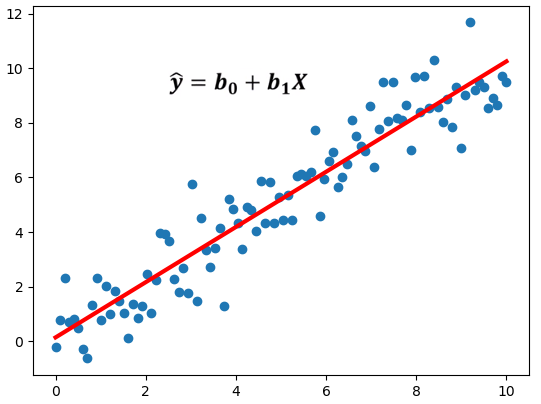
\includegraphics[scale=0.7]{Graficas/RL_1.png}
\caption{Arpoximación Lineal}
\end{figure}
\\
Durante estas notas vamos a deducir la ecuación:
\begin{equation*}
\begin{split}
\widehat{\beta}=(X^{T}X)^{-1}X^{T}Y
\end{split}
\end{equation*}
En donde X es el conjunto de datos, Y la variable dependiente, y $\widehat{\beta}$ es el vector de estimadores o pesos.
\begin{definicion}{}{}
Sea $\widehat{w}\in\mathbb{R}^{n}$ y $\widehat{x}\in\mathbb{R}^{m}$, definimos a la derivada de $\widehat{x}$ con respecto a $\widehat{w}$ como:
\begin{equation*}
\begin{split}
\frac{dx}{dw}=\left(
\begin{tabular}{ccc}
$\frac{\partial x_{1}}{\partial w_{1}}$ & $\cdots$ & $\frac{\partial x_{1}}{\partial w_{n}}$ \\ 
$\vdots$ & $\ddots$ & $\vdots$ \\ 
$\frac{\partial x_{m}}{\partial w_{1}}$ & $\cdots$ & $\frac{\partial x_{m}}{\partial w_{n}}$ \\ 
\end{tabular} 
\right)
\end{split}
\end{equation*}
es decir $\left( \frac{dx}{dw} \right)_{i,j}=\frac{\partial x_{i}}{\partial w_{j}}$
\end{definicion}
\smallskip
\begin{proposicion}{}{}
Sea $A \in M_{nxm}(\mathbb{R})$ y $w \in \mathbb{R}^m$ (o equivalentemente $w \in M_{mx1}(\mathbb{R})$). Si las entradas de $A$ no dependen de las entradas de $w$ entonces:
\begin{equation*}
\begin{split}
\frac{d(Aw)}{dw} = A
\end{split}
\end{equation*}
\end{proposicion}
\begin{proof}
$$(Aw)_i = \sum_{k = 1}^n A_{ik}w_k$$\\
Entoces:
\begin{equation*}
\begin{split}
\left(\frac{d(Aw)}{dw}\right)_{ij} &= \frac{\partial (Aw)_i}{\partial w_j}\\&= \frac{\partial \left(\sum_{k = 1}^n A_{ik}w_k\right)}{\partial w_j}\\&= \sum_{k = 1}^n \frac{\partial(A_{ik}w_k)}{\partial w_j}\\
&= \sum_{k = 1}^n A_{ik}\frac{\partial w_k}{\partial w_j}\\& = \sum_{k = 1}^n A_{ik}\delta_{kj}\\& = A_{ij}
\end{split}
\end{equation*}
Por lo tanto $$ \left(\frac{d(Aw)}{dw}\right)_{ij} = A_{ij}$$
y se concluye que:
$$\frac{d(Aw)}{dw} = A$$
\end{proof}
Para la regresión lineal vamos a utilizar la función RSS, la cual es:
$$RSS = \sum_{i = 1}^n (y_i - \hat{y}_i)^2$$

Esta función se conoce normalmente como la ``función de costo", ``loss function" o ``función de error". Nos da la suma del error cuadrático para cada una de las predicciones.
Esta sería una función que depende de los estimadores $\hat{\beta_i}$ o el vector de estimadores $\hat{\beta}$.\\
\\
Sea $X \in M_{nxp}\left(\mathbb{R}\right)$ el conjunto de datos y $\hat{\beta} \in M_{px1}\left(\mathbb{R}\right)$ el vector de estimadores, entonces:
$$\hat{y} = X\hat{\beta}$$
\begin{definicion}{RSS}{}
Podemos reescribir a RSS en forma matricial como:
$$RSS = \sum_{i = 1}^n (y_i - \hat{y}_i)^2 = (y-\hat{y})^T(y-\hat{y})$$
\end{definicion}
\begin{figure}[hbtp]
\centering
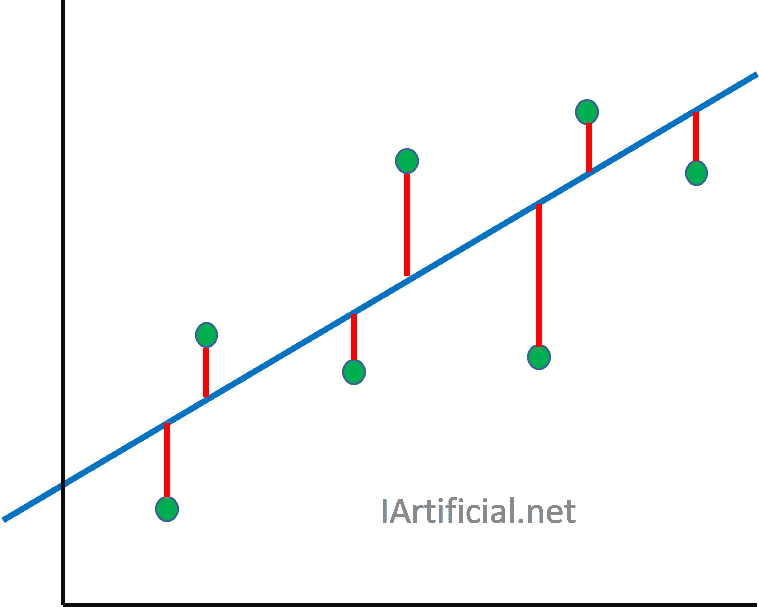
\includegraphics[scale=0.3]{Graficas/RL_2.png}
\caption{}
\end{figure}
Lo que queremos hacer es obtener los estimadores o pesos que minimicen dicha función de error.
$$(AB)^T=B^TA^T$$
\begin{proposicion}{}{}
El vector de estimadores que minimiza a RSS es:
$$\hat{\beta} = \left(X^TX\right)^{-1}X^Ty$$
\end{proposicion}
\begin{proof}
\begin{equation*}
\begin{split}
RSS &= (y-\hat{y})^T(y-\hat{y})\\&= y^Ty-y^T\hat{y}-\hat{y}^Ty+\hat{y}^T\hat{y}\\&= y^Ty-y^TX\hat{\beta}-\hat{\beta}^TX^Ty+\hat{\beta}^TX^TX\hat{\beta}
\end{split}
\end{equation*}


Derivamos la expresión anterior con respecto a $\hat{\beta}$ e igualamos la derivada a 0 para encontrar el vector de estimadores que minimiza el error RSS:
$$\frac{dRSS}{d\hat{\beta}}
=^{Proposicion\,1} -y^TX + \hat{\beta}^TX^TX=0$$
\begin{equation*}
\begin{split}
\Rightarrow &y^TX=\hat{\beta}^TX^TX\\&
\Rightarrow X^TX\hat{\beta}=X^Ty \\&
\therefore  \hat{\beta} = (X^TX)^{-1}X^Ty \\
\end{split}
\end{equation*}
\end{proof}
\end{document}